% This is samplepaper.tex, a sample chapter demonstrating the
% LLNCS macro package for Springer Computer Science proceedings;
% Version 2.20 of 2017/10/04
%
\documentclass[a4paper,12pt]{article}
\usepackage[top=1.5in, bottom=1in, left=1in, right=1in]{geometry}
%
\renewcommand{\footnotesize}{\fontsize{8pt}{9pt}\selectfont}
\usepackage{cite}
\usepackage{amsmath}
\usepackage{booktabs} % For pretty tables
\usepackage{caption} % For caption spacing
\usepackage{subcaption} % For sub-figures
\usepackage{graphicx}
\usepackage{pgfplots}
\usepackage[all]{nowidow}
\usepackage[utf8]{inputenc}
\usepackage{tikz}
\usepackage{pbox}
\usetikzlibrary{er,positioning,bayesnet}
\usepackage{multicol}
\usepackage{algpseudocode,algorithm,algorithmicx}
%\usepackage{minted}
\usepackage{setspace}
\definecolor{navy}{HTML}{000090}
\definecolor{gris}{HTML}{636F66}
%\usepackage{hyperref}
\usepackage[hidelinks]{hyperref}
\usepackage[bottom, hang, flushmargin]{footmisc} 
\hypersetup{colorlinks=true, linkcolor=navy, citecolor=navy, citebordercolor=gray}


\usepackage[round]{natbib}
\bibliographystyle{chicago}


\usepackage[inline]{enumitem} % Horizontal lists
% Used for displaying a sample figure. If possible, figure files should
% be included in EPS format.
%
% If you use the hyperref package, please uncomment the following line
% to display URLs in blue roman font according to Springer's eBook style:
% \renewcommand\UrlFont{\color{blue}\rmfamily}
\usepackage[export]{adjustbox}
%\usepackage{caption}
\usepackage[flushleft]{threeparttable}
\usepackage[page]{appendix} % print appendices title
\renewcommand{\appendixpagename}{Appendix} % Appendices title
\usepackage{array}
\usepackage{amssymb}
\usepackage{amsfonts}
%\usepackage{amsmath}
\usepackage{mathtools}
\usepackage{array}
\usepackage{subcaption}
%\usepackage{setspace}
\usepackage{adjustbox}
\usepackage{float}
\usepackage{longtable}
\usepackage{multirow}
\usepackage{tabularx, boldline}
\usepackage{cellspace}
\usepackage{booktabs}
\usepackage{soul}
\usepackage{soulpos}
\ulposdef{\hlst}{%
    \rlap{\textcolor{yellow}{\rule[-.75ex]{\ulwidth}{2.5ex}}}%
    \rule[.45ex]{\ulwidth}{.1ex}%
}

\usepackage{changepage}
\usepackage{longtable}
\usepackage{amssymb,amsmath}
\usepackage{titlesec}
\titlespacing\section{0pt}{10pt plus 4pt minus 2pt}{12pt plus 3pt minus 2pt}
\providecommand{\keywords}[1]{\textbf{\textit{Keywords --}} #1}

\newcommand{\card}[1]{\left\vert{#1}\right\vert}
\newcommand*\Let[2]{\State #1 $\gets$ #2}
\definecolor{blue}{HTML}{1F77B4}
\definecolor{orange}{HTML}{FF7F0E}
\definecolor{green}{HTML}{2CA02C}

\pgfplotsset{compat=1.14}

\renewcommand{\topfraction}{0.85}
\renewcommand{\bottomfraction}{0.85}
\renewcommand{\textfraction}{0.15}
\renewcommand{\floatpagefraction}{0.8}
\renewcommand{\textfraction}{0.1}
\setlength{\floatsep}{3pt plus 1pt minus 1pt}
\setlength{\textfloatsep}{3pt plus 1pt minus 1pt}
\setlength{\intextsep}{3pt plus 1pt minus 1pt}
\setlength{\abovecaptionskip}{2pt plus 1pt minus 1pt}
\renewcommand{\figurename}{Figure}
\def\changemargin#1#2{\list{}{\rightmargin#2\leftmargin#1}\item[]}
\let\endchangemargin=\endlist 

\usepackage{titling}
\newcommand{\subtitle}[1]{%
  \posttitle{%
    \par\end{center}
    \begin{center}\Large#1\end{center}
    \vskip0.1cm}%
}


\usepackage{geometry}
 \geometry{
 a4paper,
 total={160mm,257mm},
 left=25mm,
 top=20mm,}
\usepackage{xcolor}
\usepackage{soul}
\usepackage{array}
\usepackage{changepage}

%
\title{Does perceived labor market competition increase prejudice between refugees and their local hosts?}
\subtitle{Evidence from Uganda and Ethiopia\thanks{The proposed study is part of the project ``Global Questions on Forced Displacement and Jobs: The impact of forced displacement on labor markets in host communities'' (project supported by the World Bank). The study was pre-registered with the AEA RCT registry on January 29\textsuperscript{th} 2022 \citep{PAP2022}. We uploaded the pre-analysis plan to the registry on June 27\textsuperscript{th} 2022, before the data collection on the project ended. Data access was first granted by the World Bank in September 2022. As part of a larger project, the data was collected and used for an analysis that appears in the published World Bank book referenced as ``von der Goltz, Jan; Schuettler, Kirsten; Bousquet, Julie; Kebede, Tewodros Aragie. 2024. The Labor Market Impact of Forced Displacement: Jobs in Host Communities in Colombia, Ethiopia, Jordan, and Uganda. Washington, DC: World Bank. \href{http://hdl.handle.net/10986/40701}{http://hdl.handle.net/10986/40701} License: CC BY 3.0 IGO.'' As such, the data, including the data from the experiment, are now publicly available in the microdata library at World Bank Microdata library and can be found here for \href{https://microdata.worldbank.org/index.php/catalog/6253}{Ethiopia} and for \href{https://microdata.worldbank.org/index.php/catalog/6252}{Uganda}. The study team would like to thank the Job Group at the World Bank and Fafo Foundation for their support in implementing the survey and the proposed experiment. Anna Gasten acknowledges funding by the German Research Foundation (DFG) - project RTG 1723 in the frame of the research training group ``Globalization and Development''. We also thank  Laura Barros, Paul Glewwe, Keisaku Higashida, Marcela Iba{\~{n}}ez, Tewodros Kebede, Jason Kerwin, Krisztina Kis-Katos, Friederike Lenel, Rama Dasi Mariani, Kirsten Schuettler, Svein Erik Stave, and Jan von der Goltz for offering feedback on the study design. We are additionally grateful for comments received at the DIW 2022 Workshop on the Integration of Refugee Families in Host Countries (Berlin, Germany), the Summer Workshop on the Economics of Inter-Group Relations and Integration (Royal Holloway, UK), the 14th International Conference on Economics of Global Interactions: New perspectives on trade, factor mobility and development (Bari, Italy), the 17th AFD-World Bank International Conference on migration and development (Bologna, Italy), the 2023 Nordic Conference in Development Economics (Gothenburg, Sweden), the 2023 European Association of Labour Economics Conference (Prague, Czech Republic), the 7th International Conference ``Understanding Forced and Voluntary Migration'' (Lille, France), the 2023 German Development Economics Conference (Dresden, Germany), the 2023 International Conference on Development Economics (Paris, France), and the Joint Data Center's 2024 Conference on Forced Displacement (Abidjan, C\^o{}te d'Ivoire).}}

%
%\titlerunning{Abbreviated paper title}
% If the paper title is too long for the running head, you can set
% an abbreviated paper title here
%
\author{Julie Bousquet\thanks{FEB LICOS, KU Leuven, Belgium. Email: \texttt{julie.bousquet@kuleuven.be}.},
Anna Gasten\thanks{University of Göttingen, Germany. Email: \texttt{anna.gasten@uni-goettingen.de}},
Mark Marvin Kadigo \thanks{Institute of Development Policy (IOB), University of Antwerp, Belgium. Email: \texttt{MarkMarvin.Kadigo@uantwerpen.be}}, \\
Jean-François Maystadt \thanks{Fonds de la Recherche Scientifique – FNRS, LIDAM/IRES-UC Louvain, Lancaster University Management School, Lancaster, LA1 4YX, UK. Email: \texttt{jean-francois.maystadt@uclouvain.be }}, and
Colette Salemi \thanks{University of Victoria, British Columbia, Canada. Email: \texttt{csalemi@uvic.ca}}}

\begin{document}


\maketitle           

\normalsize
\singlespacing

\pagebreak

\begin{abstract}

\noindent We study whether perceptions of labor market competition negatively influence out-group attitudes between refugees and their local hosts using a survey vignette experiment conducted in urban and rural Ethiopia and Uganda. Our vignette consists of a short story about a fictional job-seeker in which we randomize the citizenship (refugee/national) and occupation (same as/different from respondent). Our estimates suggest that host attitudes are significantly more negative when the vignette character is a refugee in the same occupation. Such prejudice against the out-group is not confirmed among refugees. Exploring the context-dependency of our results, evidence suggests that negative attitudes toward refugees that are tied to perceived labor market competition largely manifest in contexts of limited refugee worker presence. Hence, perceived labor market competition contributes to prejudicial attitudes, but results suggest that these perceived threats do not necessarily coincide with experienced labor market competition between refugees and their hosts. Additional heterogeneity analysis based on prior contact and ethno-linguistic proximity provides suggestive evidence that cross-group interactions reduce the salience of perceived labor market competition as a driver of out-group prejudice in refugee settings. \\


\bigskip

\noindent \keywords{Refugee hosting; Ethiopia; Uganda; Vignette experiment; Prejudice; Labor markets}

\end{abstract}

\setcounter{footnote}{0} 

%
%
%
\pagebreak

\onehalfspacing

%%%%%INTRODUCTION

\section{Introduction}

\noindent Many of the 30 million refugees around the world are experiencing long-term displacement and are unlikely to return to their home country in the foreseeable future \citep{milner2011responding}. Given the low probability of resettlement to a wealthier host country, most (75\%) refugees remain in a low- or middle-income host country \citep{UNHCRreport2024}, residing either in a refugee camp adjacent to communities from the host country (henceforth ``host communities'' or ``hosts'') or among their hosts in an out-of-camp context. For these refugees, integrating into host community markets and society is crucial for improving the household's welfare and reducing their dependence on humanitarian assistance \citep{clements2016uganda, coate1993, glover2017}. While many host country governments promote integration through liberal refugee hosting policies \citep{UNHCRDurable, blair2022}, public antagonism towards refugees may negatively impact hosts' willingness to include refugees in society \citep{loiacono2019improving}.


We conduct a survey experiment in Uganda and Ethiopia to examine the role of perceived labor market competition in mediating inter-group attitudes in refugee hosting contexts. Our experiment consists of a vignette embedded in the Harmonized Host and Refugee Labor Market Survey (HHR-LMS) collected by the World Bank Group and Fafo in 2022. Within the vignette, we randomize two key attributes of the vignette character: whether the vignette character is a citizen or a refugee, and whether the vignette character works in the same occupation as the respondent or in a different occupation of similar education level. After exposure to the vignette, respondents (refugees or hosts) answer questions that gauge their attitudes about the vignette character. We use an OLS regression approach to examine differences in self-reported attitudes towards members of a respondent's out-group relative to attitudes towards members of the respondent's in-group. In this context, a host (refugee) respondent's in-group consists of other hosts (refugees), and a host (refugee) respondent's out-group consists of refugees (hosts). Our objective is to understand not only how out-group versus in-group attitudes differ, but whether perceived labor market competition (proxied by an out-group member working in the same job as the respondent) matters in determining out-group attitudes.

We collected our survey and vignette data in four locations of rural and urban Uganda and Ethiopia, as shown in \hyperref[fig:map]{Figure} \ref{fig:map}. At the time of our study, these two countries are hosting the largest refugee populations in sub-Saharan Africa (1.5 million in Uganda and 823,000 in Ethiopia) \citep{UNHCRreport2021}. Uganda had a more open hosting policy, granting refugees the right to work and move within the country without encampment requirements. In Ethiopia, although refugees theoretically enjoyed similar rights, practical restrictions were more significant \citep{UNDP2017Uganda, UNHCR2020ecrrp, betts2022states}. At the time of the study, the Tigray War was ongoing in Ethiopia, resulting in large-scale internal displacement, including refugees fleeing refugee camps located in the Tigray region \citep{tsegay2023internal}. In both settings, the majority of refugees live outside of the capital cities under a system of encampment: in Ethiopia, this takes the form of small-area camps, while Uganda provides large-area refugee settlements in which refugees are allocated small agricultural plots. The diversity of settings studied in Ethiopia and Uganda helps us examine some of the context-specific conditions that could reinforce out-group prejudices.

\vspace{5mm}

\begin{figure}[h]
        \footnotesize
        \captionsetup{width=1\linewidth}
        \caption{Map of study locations}
        \label{fig:map}
         \centering
        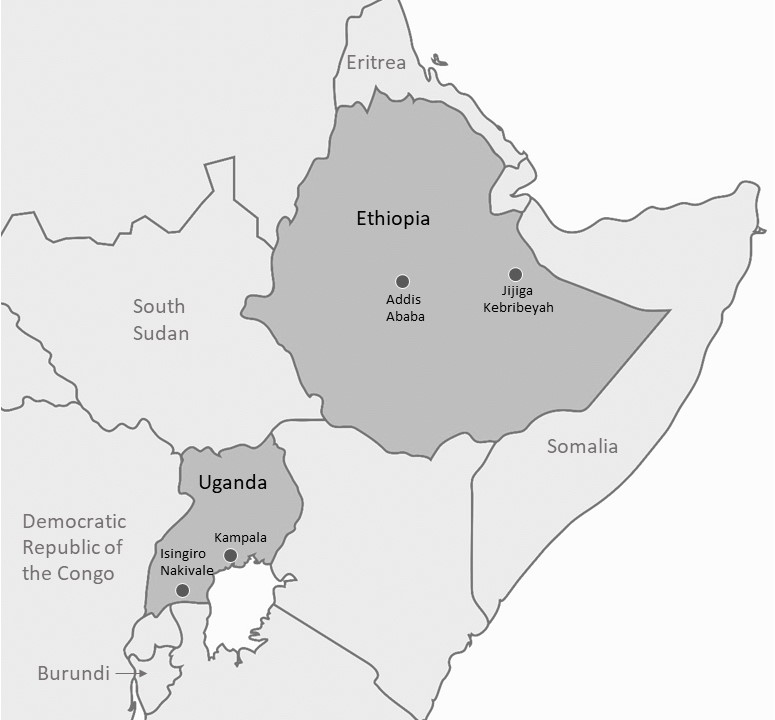
\includegraphics[height=0.6\textwidth]{Figures/FIG1_Map_Ethiopia_Uganda.jpg} \\
\end{figure} 

\vspace{5mm}
    

    
Overall, we find that hosts hold more negative attitudes towards refugees compared to their attitudes towards other hosts, but only when sharing the same occupation. Decomposing our estimates by region, the negative reaction to a refugee character working in the same occupation is driven by host respondents in Addis Ababa, Ethiopia. In Isingiro/Nakivale (Uganda), negative attitudes towards refugees are reported regardless of labor market concerns. We further disentangle our findings through a heterogeneity analysis examining the role of cultural diversity, intergroup contact, and industry-location labor market characteristics across the four contexts.

Our results indicate that perceived labor market competition plays a more significant role in intensifying prejudice against refugees for host respondents in competitive labor markets (from the perspective of workers). Moreover, we find that perceived competition is only tied to prejudice among workers in local industries with low refugee representation. The latter result suggests that misconceptions of refugees as job competitors negatively impact host views of refugee out-groups, aligning with other cases in which prejudicial beliefs about out-groups do not fully align with reality \citep{allport1954nature}. Further analysis exploring variations based on prior interpersonal interactions and cultural similarities implies that inter-group engagements and cultural commonalities correlate with a reduction in out-group prejudice driven by perceived labor market competition.

Our study contributes to multiple discourses related to migration, out-group attitudes, and inter-group contact. First, past scholarship has debated whether anti-migrant prejudice is motivated by private economic concerns, such as anxieties over competition for jobs \citep{muller2020individual, mayda2006against} or sociotropic concerns, such as fears over the ``identity of the nation'' changing due to migration \citep{hainmueller2010attitudes, hainmueller2014public}. Our work offers evidence that perceived, but likely unrealized economic competition influences anti-immigrant attitudes \citep{dennison2018}.
Secondly, we indirectly contribute to a recent literature that has explored the role of inter-group contact in improving attitudes and behaviors toward the outgroup \citep{lowe2021, mousa2020building, scacco2018can, betts2023refugees}. This research is informed by the ``Contact Hypothesis'' first proposed by \citet{allport1954nature} and supported by \citet{pettigrew2006meta} and \citet{paluck2019contact}. We descriptively show that the negative reaction to a refugee character holding the same occupation is driven by hosts who report limited contact with refugees.

Our findings also extend previous research on ethno-linguistic proximity between refugees and the host population. Existing studies suggest that ethnic diversity limits support for refugees, a concept known as the ``group threat hypothesis'' \citep{steele2019ethnic}.  Conversely, greater ethno-linguistic proximity is associated with more positive attitudes of hosts towards refugees \citep{betts2023refugees}. 

Finally, we consider a dimension of inter-group attitudes in forced displacement settings previously unexplored: attitudes among refugees towards their hosts and each other. Such a perspective may shed light on the way members of minority groups may hold prejudice not only against the majority group but also against members of their own groups \citep{perlmutter2002}. Our full results suggest that refugees do not hold more negative attitudes towards the vignette character when the character was a host community member, regardless of perceived labor market competition. But given small sample counts for refugees in some study sites, additional mediation analyses by locality are frequently under-powered. 

Our paper proceeds as follows. Section 2 describes the knowledge discourses that our work builds on in greater detail. Following this, we provide contextual information about our study sites in Section 3. In Section 4, we describe our data and the design of our survey vignette and randomized experimental procedure. We introduce our estimation methodology in Section 5, and in Section 6, we explore our overall results, as well as important heterogeneity. Section 7 contextualizes our results within the local landscapes, while also discussing potential underlying mechanisms. We conclude in Section 8. 


%%%LIT REVIEW


\section{State of knowledge}

\noindent Our work is motivated by the ongoing discourse on the labor market impacts of refugee hosting. When expressing grievances over the consequences of displacement, local host communities have often stressed rivalry over job opportunities and other scarce resources \citep{baylouny2020, fajth2019}. Because of these concerns, the impact of refugees on host labor markets has received considerable scholarly attention in recent years \citep{aksu2022, caruso2021, maystadt2014winners, ruiz2016labour, fallah2019impact}. While the labor market impacts are often small or null, certain host sub-groups are more negatively affected than others \citep{maystadt2014winners, ruiz2018, Goltz2023jobs}. 

The study also contributes to several important research areas related to migration, out-group perceptions, and societal harmony. First, our work corresponds to the discourse on prejudicial attitudes towards out-group members in migration settings. We follow past studies on forced displacement  \citep{hangartner2019does, adida2018perspective, hatton2017refugees}, but given ambiguities in delineating migration that is voluntary versus involuntary \citep{bakewell2021unsettling}, we align our work with the voluntary migration discourse as well.  Studies of anti-migrant attitudes evaluate whether private economic concerns or sociotropic factors are more influential in fueling negative attitudes towards migrants. Private economic factors include perceived threats to an individual's income and wealth, either because the individual believes that migrants represent increased job competition or that state services for migrants will increase their tax burden \citep{muller2020individual}. Studies examining personal economic factors often compare attitudes among hosts depending on skill level. If private economic concerns fuel anti-migrant attitudes, then one would expect that low-skilled hosts are more likely to feel threatened by low-skilled migrants \citep{hainmueller2010attitudes, mayda2006against}. 

The results of past studies on the private economic determinants of anti-migrant attitudes have been mixed. For example, \cite{mayda2006against} provides descriptive evidence that prejudice against low-skill migrants attenuates in countries with a large share of high-skill workers, suggesting that private threats of job competition are an important determinant of prejudice against migrants. By contrast, \cite{hainmueller2014public} argue that anti-migrant attitudes often manifest among low-skilled and high-skilled hosts, weakening the hypothesis that private economic factors fuel prejudice. Through their online survey in high-income countries, \citet{valentino2019} reject hypotheses based on narrow economic threats, either through labor market competition, perceptions of higher tax burden or threats to welfare benefits. In the context of post-Apartheid South Africa, \citet{facchini2013} found that labor markets are not likely to explain the observed variation in individual attitudes towards immigration. Ethnicity or religion are stronger drivers of individual attitudes.  

We build on this discourse by examining low-income country contexts in which refugee and host skill sets may be more similar and markets are incomplete. With few exceptions \citep{mayda2006against, facchini2013}, the past work on anti-migrant prejudice has focused on wealthy country contexts. In high-income countries, low-skilled migration often does not lead to economically meaningful increases in unemployment or lower wages for hosts. Scholars have argued that losses for low-skilled host workers do not manifest because low-skilled migrants serve as a substitute for capital investments \citep{clemens2018immigration} and/or because firms upgrade low-skill host workers to more managerial tasks \citep{foged2016immigrants}. 

But in low-income countries like Uganda or Ethiopia, domestic workers tend to have less specialized skill sets, so refugee labor may serve as a substitute for the labor of certain segments of the population. Moreover, constraints on savings and investment limit the substitutability between capital and low-skilled labor and the potential skill upgrading of hosts. As a result, local workers may feel threatened by the influx of new arrivals who are seen as direct competitors for jobs. Additionally, the weakness of social protection systems may make economic concerns more salient \citep{alrababa2021attitudes, becker2022}. 

When studying attitudes towards migrants and private economic concerns, it is important to consider whether perceived concerns represent real phenomena. There is suggestive evidence that the perception of refugees ``stealing jobs'' may persist even in contexts where the labor market effect of refugees on hosts may be small or nil. For instance in Jordan, it has been argued that refugees primarily compete with migrant workers in the labor market \citep{fallah2019impact, assaad2019structure}, while the public perception is still that refugees are replacing Jordanian workers \citep{baylouny2020}. Our study offers insights into the relationship between perceived, but not realized, competition over jobs and anti-migrant attitudes.  

Past research on anti-migrant attitudes has also examined the role of ``sociotropic'', or ``sociopsychological'' factors. Such factors include beliefs regarding national identity, the value of diversity, etc. Several studies have argued that these sociotropic factors are a strong predictor of prejudice against migrants \citep{hainmueller2014public, card2012immigration, valentino2019}. But as with the private economic concerns hypothesis, the majority of past work has focused on high-income country settings. Recent scholarship has argued that sociotropic concerns are less important in low-income countries given the weakness of the welfare state and higher cultural heterogeneity \citep{alrababa2021attitudes, becker2022}.\footnote{One possible exception is South Africa \citep{facchini2013}.} Our study does not directly test sociotropic factors and their relationship to prejudice in refugee settings, but by focusing on private economic concerns, our study still contributes to the overall understanding of anti-migrant attitudes. 

Our methodology draws insights from past work using vignettes to develop our experiment. The vignette we designed is intended to solicit, but not transform, respondent attitudes about the out-group. As opposed to conventional conjoint experimental methodologies, which are commonly used to gauge the relative importance of various attributes of a hypothetical individual presented in table format \citep{alrababa2021attitudes, hainmueller2014causal, becker2022}, we use a one-shot narrative vignette.  This approach allows us to embed randomized elements within an engaging story and to measure how this implicit treatment influences subsequent responses in the survey. 

Previous studies have used vignette experiments to understand and attempt to change negative out-group perceptions. These studies often use simulations or stories intended to help respondents empathize with the experiences of a vulnerable out-group \citep{rodriguez2021attitudes, adida2018perspective,  cattaneo2021turning, simonovits2018seeing, chatruc2024}. In some cases, the vignette is intended to remind or inform respondents of an important characteristic that the respondent shares with the out-group, such as belonging to the same religious sect \citep{lazarev2017brother} or sharing a family history of forced displacement \citep{dinas2021family}. Vignettes have also been used to expose survey respondents to more accurate information about migrants \citep{blinder2020going, grigorieff2020does, haaland2020labor, hopkins2019muted, facchini2022countering}. Such interventions have been shown to improve respondents' stated willingness to engage with the out-group, but only along certain social dimensions, and the impacts may be short-lived. Our approach is similar to \cite{lazarev2017brother}, but instead of focusing on a cultural commonality across groups, we explore the differences in attitudes when the groups share occupational characteristics, which may represent competition instead of accord. 

Additionally, our work contributes to the study of social cohesion and local integration in refugee hosting or post-conflict settings.  Several past studies have stimulated inter-group contact  to see if greater exposure to out-group members improves attitudes and behaviors toward the out-group \citep{lowe2021, mousa2020building, scacco2018can, betts2023refugees}. For example, based on observational data, Lebanese respondents exhibit favorable attitudes towards refugees if they reported recent contact with Syrian refugees \citep{ghoshn2019}. Recent work by \cite{barros2023power} finds that repeated dialogue through joint community meetings improved relations between internally displaced persons and hosts in Mozambique. 

Others have studied the impact of cash transfers to refugees and hosts on social cohesion. When cash transfers are targeted at both groups, refugee recipients' willingness to engage with the host community increases, but cash transfers have a limited impact on improving host attitudes towards refugees \citep{valli2019economic}. When the hosts receive cash transfers in Uganda, in particular when framed as tied to the refugee policy, they tend to hold favorable attitudes towards refugees \citep{baseler2022can}. And when cash transfers target refugees only, evidence suggests that hosts do not become more hostile towards refugees \citep{lehmann2020}.  While cash for refugees may not lead to violence between groups, encouraging prosocial behavior between groups may require a better understanding of inter-group prejudice.  


Finally, our examination of in- vs. out-group attitudes among refugees corresponds to a small discourse on the ways in which refugees perceive other refugees. Past qualitative work on refugees in Nakivale has noted longstanding frictions between different ethnic or national groups \citep{bjorkhaug2020revisiting}. Recent work has also considered how past displacement experiences influence current attitudes towards new refugee arrivals \citep{gihleb2022exposure}. 

    
\section{Context}


The study focuses on refugee-hosting areas in Uganda and Ethiopia, two of the three countries in Sub-Saharan Africa (SSA) with the largest refugee populations. Uganda and Ethiopia, like several other East African countries, have a longstanding history of hosting refugees and generally maintaining an open-door approach towards refugee arrivals \citep{UNHCR2022RSS, UNHCR2020OPM}. Additionally, both countries host refugees facing protracted displacement, commonly referred to as a condition where refugees have resided in the host country for a duration of five years or longer \citep{milner2011responding}. For these refugees, voluntary return to their home country is often unfeasible in the near future, further necessitating local inclusion efforts. 


With approximately 1.5 million refugees being hosted, at the time of the survey, Uganda hosted the largest refugee population in Sub-Saharan Africa and the third highest globally \citep{UNHCRreport2021}. Refugees in Uganda come primarily from South Sudan, the Democratic Republic of Congo, Burundi, Somalia, Rwanda, Eritrea, and Ethiopia. Instead of relying on geographically small camps, Uganda uses a model of hosting refugees in settlements, designating a total of 13 settlements of considerable land area. 

Nakivale settlement, evaluated as part of this study, is one of Uganda's oldest refugee settlements. Located in the southwestern Isingiro district, Nakivale was officially recognized as a settlement in 1960 and allocates about 185 $km^2$ for refugees \citep{bjorkhaug2020revisiting}. Isingiro district and the Nakivale settlement primarily host refugees from the Democratic Republic of Congo, Rwanda, Burundi, Eritrea, Ethiopia, and Somalia. Thus, this context is characterized by a diverse profile of refugees living alongside Ugandan nationals. To augment social integration in settlement areas, health, education, and other welfare-enhancing services for refugees are shared with hosts, resulting in improved public service delivery \citep{zhou2022inclusive}. Refugees in settlements systematically receive humanitarian aid.

Uganda's refugee hosting policies emphasize refugee self-reliance \citep{clements2016uganda, betts2023refugees}. Refugee households that reside in settlements receive land for cultivation, providing opportunities for agricultural subsistence or market activity \citep{betts2017refugee, betts2019refugee, kadigo22}. The rights of refugees in Uganda were extended by the Uganda Refugee Act of 2006. This legislation, along with its associated policies and regulations, grants refugees the freedom of movement, access to social services provided by the country, and the freedom to seek employment or establish their own businesses. Due to this freedom of mobility, a considerable proportion of the refugee population resides outside of planned refugee settlements \citep{UNDP2017Uganda, KampPop2022}. With about 6\% of the total Ugandan refugee population, Kampala district hosts the highest number of urban refugees. The overall refugee population residing in Kampala was slightly increasing over the five years leading up to the survey, with 98,000 refugees registered in 2017 and 114,000 by April 2022 \citep{saliba2020cities, KampPop}. At the time of the survey, refugees represented about 3.1\% of the population residing in the Kampala metropolitan area, which totals about 3.7 million people \citep{WorldPopReviewKampala}. Refugees in Kampala are self-settled in scattered locations but usually concentrated in particular areas that form neighborhoods of refugees from the same country. For instance, Congolese and South Sudanese refugees are concentrated in Katwe and Nsambya, Eritrean and Ethiopian refugees in Kabalagala, Somali refugees in Kisenyi and Burundi and Rwanda refugees in Nansana and Namungoona. 

These self-settled refugees are usually registered as urban refugees and therefore are not entitled to the humanitarian aid provided to those in the settlements. Some endure difficult living conditions, often settling in Kampala's slums among the urban poor. Nonetheless, the registered urban refugees can benefit from free access to some essential services (such as medical services) and can be beneficiaries from targeted development projects. 

Given the opportunities offered to refugees and the use of inclusive services to improve social harmony, Uganda has been praised for advancing a set of refugee management policies aimed at improving local inclusion of refugees. But critics have pointed out that these efforts can only go so far in fostering self-reliance and inclusion. For example, studies of the land allocation policy have argued that the policy may not truly foster self-reliance due to poor land quality, limited land quantity, and the challenges refugees face when trying to get their agricultural products to market \citep{bohnet2019uganda, kaiser2006between, betts2019refugee}. Moreover, descriptive and qualitative studies of urban refugees in Uganda provide evidence of discrimination and prejudice \citep{hook2015sharing, stark2015he}, suggesting that policies toward improving relations between refugees and host communities in some settings cannot completely prevent bias. 

\vspace{5mm}

              \begin{center}
\begin{figure}[H]
	\footnotesize
          \caption{Map showing study sites and sampled households in Uganda}
          \label{fig:map_uganda}
          \centering
		%\begin{adjustwidth}{0cm}{}
        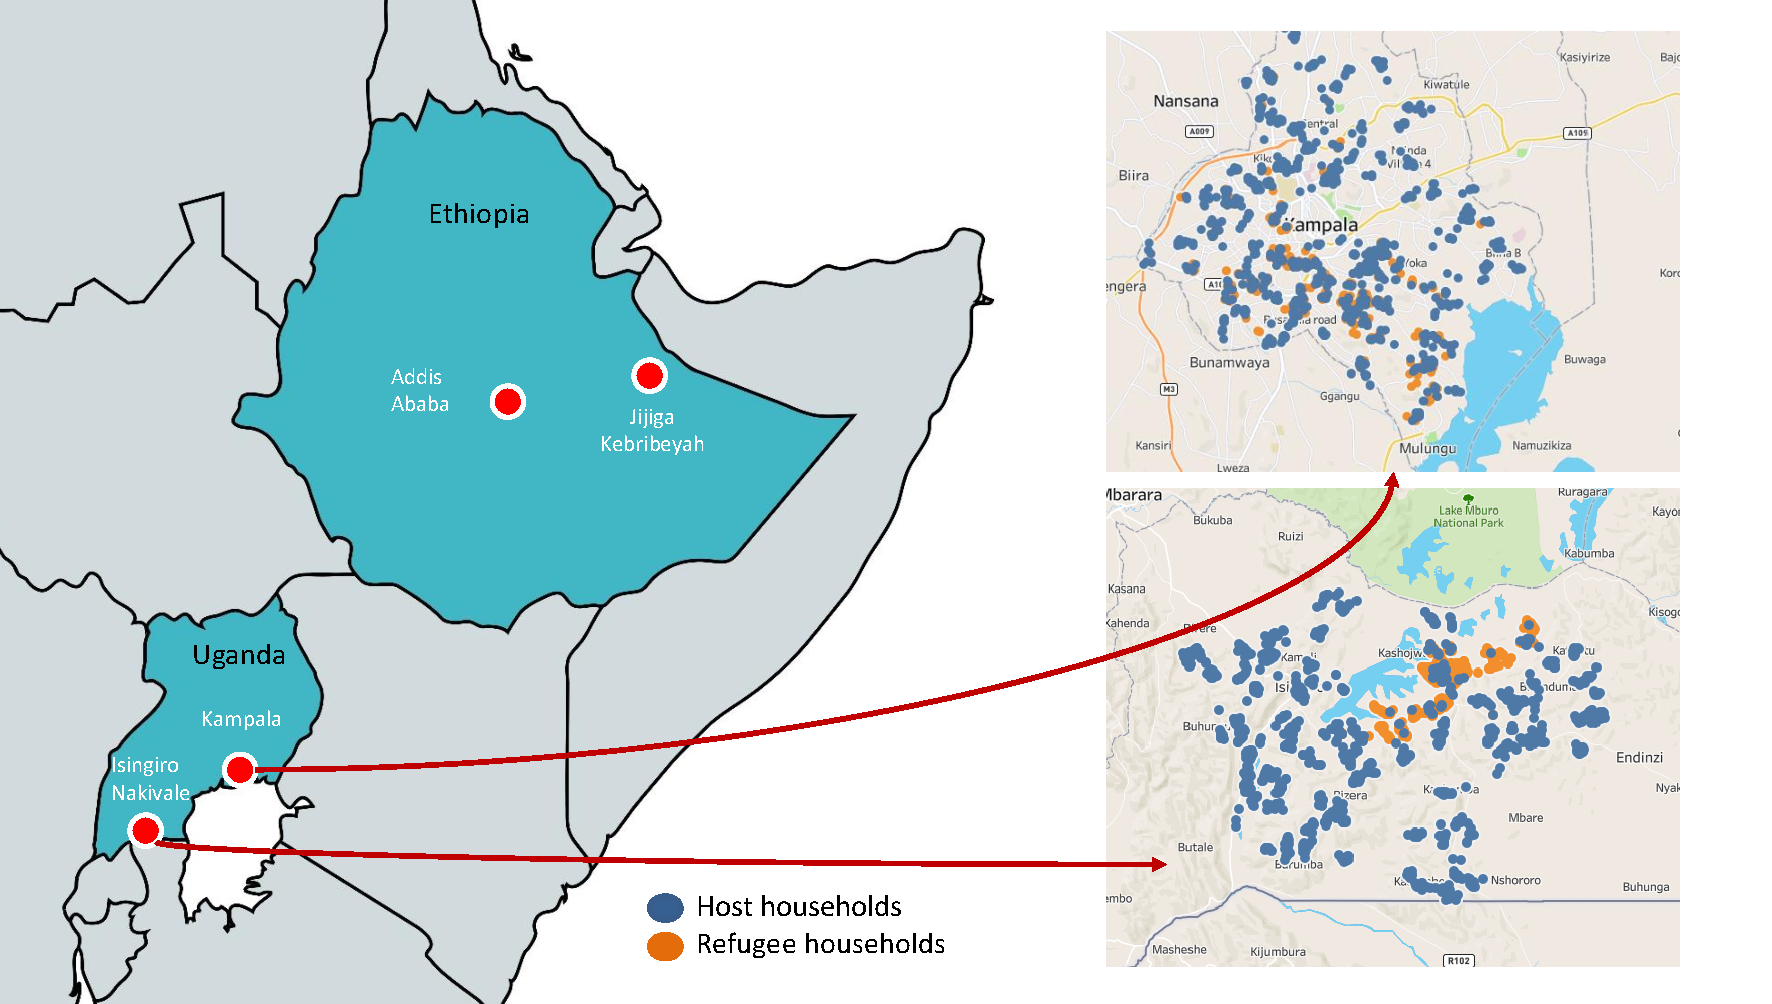
\includegraphics[height=0.6\textwidth]{Figures/FIG2_Map_Uganda.pdf} \\
        \begin{minipage}{0.65\textwidth}
 { \footnotesize Source: Authors' formulation supplemented by data from the World Bank. \par}
\end{minipage}
 \end{figure} 
\vspace{5mm}
   \end{center}
   
  
    
Ethiopia is home to the third largest refugee community in Sub-Saharan Africa, and at the time of survey, Ethiopia ranked ninth globally, accommodating approximately 823,000 refugees \citep{UNHCRreport2021}. The refugee population is predominantly from South Sudan, Somalia and Eritrea. Historically, Ethiopian refugee hosting policies were highly restrictive: With few exceptions, refugees were required to live within camps and refugee labor was prohibited \citep{betts2019Addis}. Although this framework was not conducive to refugee integration, inclusive services at camp locations were designed to be shared with hosts \citep{jahre2018approaches}, which may have served to abate anti-refugee sentiments. 
    
In recent years, Ethiopia's strict rules were increasingly relaxed. In 2010, the country began allowing Eritrean refugees who were not dependent on humanitarian assistance to settle outside camps \citep{abebe2018promises, betts2023refugees}. On 17 January 2019, the Ethiopian Parliament revised its refugee laws. Because of these amendments, all refugees are now granted access to a wide range of nationally provided services, have the right to work and own property, and have freedom of movement, among other provisions \citep{UNHCR2020ecrrp}. As such, refugees were able to relocate to areas outside of camps during the period that preceded the collection of the data used in this study, though many refugees also remained in camps.  
   
The ongoing conflict in the Tigray region of Ethiopia has impacted the distribution of refugee populations over the country. Many refugees (especially Eritreans) have fled from Tigray to Addis Ababa, resulting in a rapid increase of the refugee population in the capital between January 2021 and July 2022. In 2022, Addis Ababa accommodated approximately 72,000 refugees, constituting around 1.4\% of the city's local population \citep{ethiopiaStatsNov22, WorldPopReviewAddis}. This marked a substantial rise of nearly 350\% within five years, compared to the approximately 21,000 refugees residing in the capital in 2017 \citep{AddisPop17}. Despite the greater relative increase in refugees residing in Addis Ababa over the past five years compared to Kampala, the total number and their proportion relative to the local population still remain significantly lower.


\vspace{5mm}

              \begin{center}
\begin{figure}[H]
	\footnotesize
          \caption{Map showing study sites and sampled households in Ethiopia}
          \label{fig:map_ethiopia}
          \centering
		%\begin{adjustwidth}{0cm}{}
        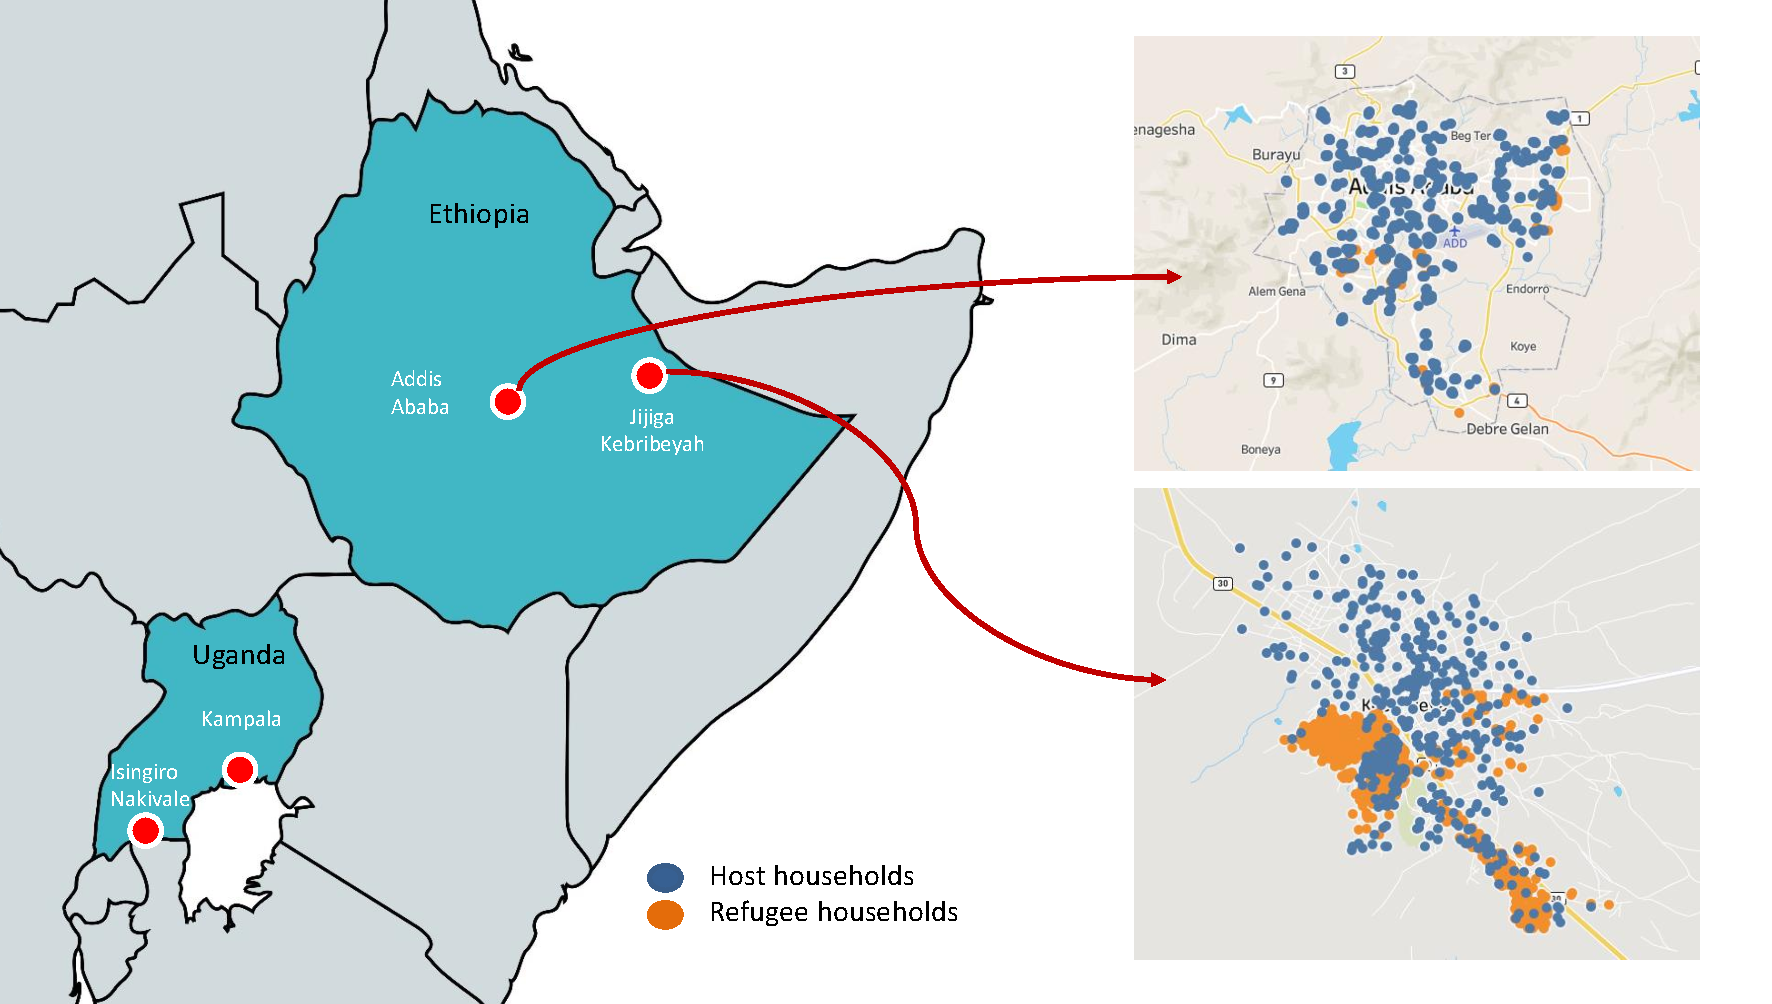
\includegraphics[height=0.6\textwidth]{Figures/FIG3_Map_Ethiopia.pdf} \\
        \begin{minipage}{0.65\textwidth}
 { \footnotesize Source: Authors' formulation supplemented by data from the World Bank. \par}
\end{minipage}
\vspace{5mm}
 \end{figure} 
   \end{center}


\section{Data}

The research design and all statistical tests have been pre-specified in a pre-analysis plan registered with the AEA RCT registry \citep{PAP2022} before data collection ended and starting data analysis. We describe any deviation from this pre-analysis plan in Appendix Section \ref{A1 Dev from PAP}. We embedded our experiment in the Harmonized Host and Refugee Labor Market Survey (HHR-LMS) collected from January 2022 to July 2022 in Uganda and Ethiopia. In Uganda, we sample hosts and out-of-camp refugees in urban Kampala ($N = 889$ hosts, $458$ refugees), refugees in Nakivale settlement ($N =702$), and hosts near Nakivale in the Isingiro district ($N = 660$). Our urban Ethiopia sample is drawn from Addis Ababa ($N = 1,219$ hosts, $198$ refugees). We also sample refugees in Kebribeyah camp ($N=301$), and Ethiopian hosts in and nearby the nearby rural town Kebribeyah within the Jijiga zone ($N=199$). The samples were drawn to represent the refugees and host populations in the two urban and two rural settings. For the host respondents, we find that our sample closely aligns with households surveyed in the same four sub-regions by the nationally representative LSMS surveys - the 2021/2022 Socio-Economic Panel Survey for Ethiopia and the 2019/2020 Uganda National Panel Survey (Table \ref{tab:summary_stats}). We describe our sampling frame in greater detail in Appendix Section \ref{sec:Sampling and data collection}.

 

Our vignette exposes respondents to a narrative describing a fictional character looking for a job. We modify certain words in the vignette to align with or differ from the respondent's occupation as well as citizenship status (refugee or host). The occupation wording uses either a shortened string of the respondent's own occupation, or a randomly drawn occupation of a pre-specified list of twelve plausible occupations, always matching the respondent's own education level. Matching with the respondent's own education level narrows the list of possible occupations to five as shown in Table \ref{tab:occupationskills}. The restricted list by education level is therefore comprised of occupations ranked at a similar skill level, so workers may switch or substitute between these roles. Consequently, our experiment compares reactions to a vignette character in the same occupation vs. a relatively similar occupation, and the counterfactual occupation may be a role the respondent is qualified to perform or has worked in before. While this job substitutability may represent a limitation of our study, we believe that this design is necessary to avoid priming respondents on differences in social class or status. 

The occupation and citizenship status are randomly assigned across four treatment groups (Table \ref{tab:treatarm}). The gender and residence of the fictitious character always align with the one of the respondent. More information is given in Appendix Section \ref{sec: additional experiment}. The narrative takes the following form in Uganda (symmetrically for Ethiopia): \\
    
    \begin{adjustwidth}{0.8cm}{0.8cm}
        \noindent 
        ``[AIDA/ROBERT] is a [GROUP: Ugandan/ refugee living in Uganda]. [She/He] (has lived in Uganda [her/his] entire life and) moved to [Isingiro district/Kampala] five years ago. [She/He] has been working as a [OCCUPATION: String of same/ different occupation as respondent] for a long time so [she/he] has a lot of experience in [her/ his] occupation. [She/He] also speaks many Ugandan local languages and English very well. [She/He] enjoys working in this profession and would recommend [her/his] friends to work in the same sector. But while being a [OCCUPATION: String of same/ different occupation as respondent] fulfills [her/him], [she/he] is sometimes very tired after work.  Due to difficult circumstances, [she/he] has to change jobs while keeping her/his current profession. So far, she/he has struggled finding a job.'' \\
    \end{adjustwidth} 

\noindent   
Immediately following the vignette, the respondents replied to questions that made them relate to the story (``What would you recommend Aida/Robert to do?'') and to a set of questions meant to gauge their self-reported attitudes towards the fictitious character. These include questions on social inclusion (feeling comfortable interacting with the character), private interactions (accepting someone like the character as a neighbor or spouse of a family member) and labor market inclusion (respondent's willingness to work alongside or for the character). As described in detail in Appendix Section \ref{sec: Anderson desc}, we use the self-reported attitudes towards the vignette character, measured on a 5-point Likert scale, to construct a prejudice index using the method introduced by \citet{anderson2008multiple}. Higher values of that index indicate more negative views toward the fictitious character. We consider disparities in attitudes by group membership to be evidence of prejudice, understood as a ``negative bias toward a social category of people'' \cite[p. 340]{paluck2009prejudice}. To examine out-group attitudes in further detail, we additionally generate three separate indices for work, private, and social interactions respectively, which allows us to examine what types of out-group interactions drive our main results within the pooled index.


\section{Method}

Our research design allows us to examine three different hypotheses. Hypothesis 1 (H1) is that both host communities and refugees hold more prejudicial views against members of the out-group, compared to members of the in-group. Examining H1 requires that we compare self-reported attitudes towards vignette characters who are out-group members versus in-group members, regardless of the occupation of the vignette character. Hypothesis 2 (H2) is that perceptions of labor market competition may have adverse effects on the views of others, independent of their group membership. We explore this hypothesis by examining how respondents react to vignette characters with the same occupation versus a different one, holding the vignette character's status (refugee or citizen) constant. Hypothesis 3 (H3) is that prejudice against members of the out-group is more pronounced when perceptions of labor market competition are strong. H3 is our hypothesis of primary interest and analyzes whether prejudice against the out-group members is driven by private concerns of livelihood losses. 

We use the experimental randomization and prejudice index to estimate the following Ordinary Least Squares (OLS) regression for refugees and hosts separately:
\begin{equation} 
\label{eq:mainspe}
\begin{split}
    Y_{i} = \alpha_{0} + \alpha_{1} OutGroup_{i} + \alpha_{2} SameOcc_{i}  
    +  \alpha_{3} OutGroup_{i} \times SameOcc_{i} + X_{i}^{'} \gamma + u_{i}
\end{split}
\end{equation} 

\noindent
The dependent variable, denoted as $Y_{i}$, captures prejudice directed toward the fictional character in social, private, and work-related contexts. This composite measure (Anderson index) standardizes the six prejudice-related questions. It exhibits a mean of zero and a standard deviation of one, offering a normalized view of prejudice levels across the various dimensions. 
$SameOcc_{i}$ is a binary indicator of whether the vignette character has the same occupation as the respondent, and $OutGroup_{i}$ is a binary indicator of whether a host (refugee) respondent is matched to a vignette character who is a refugee (host). The interaction $SameOcc_{i} \times OutGroup_{i}$ indicates whether the vignette character is both an out-group member and in the same occupation as the respondent. The intercept ($\alpha_{0}$) represents the average index score for those exposed to a vignette character who is an in-group member working in a different occupation. 

The coefficients of this specification require particular care in translating.  The $\alpha_{1}$ coefficient estimates the effect of exposure to a vignette character in the respondent's out-group who is working in a different occupation, relative to a vignette character from the respondent's in-group working in a different occupation. It is important to note that this estimate represents differential reactions from respondents who are all assigned to a vignette character working in a different occupation. The $\alpha_{2}$ coefficient represents the effect of exposure to a vignette character in the respondent's in-group who works in the same occupation as the respondent, relative to an in-group vignette character working in a different occupation. This estimate only reflects the outcomes for respondents matched to an in-group character. Finally, $\alpha_{3}$, our coefficient of primary interest, directly tests hypothesis H3.  It reports the effect of exposure to an out-group member in the same occupation relative to all other treatments. We cluster our standard errors at the enumeration area level in accordance with our two-stage sampling design \citep{abadie2017should}. 

To examine H1, we must evaluate the combined effects of exposure to an out-group member regardless of their occupation. Likewise, examining H2 requires we isolate the impact of exposure to a vignette character with the same occupation, regardless of whether they are a host or refugee We do so by determining the partial effects, which we report consistently throughout the Appendix.\footnote{In the Appendix tables of regression outcomes, these partial effects are labeled as H1 and H2, respectively.}

Since randomization is implemented at the individual level, the treatment assignment is expected to be uncorrelated with the individual characteristics of respondents. Balance tests reported in Appendix Section \ref{sec: additional descriptives} (Table \ref{tab:balance}) demonstrate that randomization created four comparable treatment groups, with only a few imbalances that do not exceed the extent we would expect under random assignment. Following the pre-analysis plan, we control for a vector of demographic characteristics, $X_{i}$, including the country of residence, location of the household (urban or rural), gender and age of the respondent, whether the respondent attained at least primary education, and their employment.\footnote{Our main results remain qualitatively identical, and quantitatively robust when omitting these control variables. The coefficients exhibit minimal variation (with effect sizes decreasing by less than 0.03 standard deviations), and the significance levels our estimates of interest remain consistent.}
We report descriptive statistics for dependent, explanatory and control variables in Tables \ref{tab:sumstat_byR_uga} and \ref{tab:sumstat_byR_eth}. 


Reactions to a vignette character with the same occupation as the respondent help us understand whether the respondent's attitudes are shaped by perceptions of higher labor market competition. By contrast, when the vignette character is in a different occupation, we consider the hypothetical context to be one of lower perceived labor market competition. Our results provide evidence of prejudice if respondents systematically report more negative social attitudes towards the vignette character when he or she is from a certain group (hosts or refugees). Since all other attributes of the fictional character are held constant, we believe that such an attitudinal asymmetry is evidence that respondents subjectively hold negative beliefs towards this group. To evaluate our assumption that the vignette character working in the same occupation invokes a sense of job rivalry among respondents, we test whether the treatment arm ``same occupation'' indeed induces a higher level of perceived labor market competition. Using an index of labour market competition as the outcome variable (constructed from 2 questions; \textit{``(1) Do you feel in competition with Aida/Robert?''} and \textit{``(2) Do you think Aida/Robert might take away your job?''}), we observe that respondents who were exposed to a narrative with ``same occupation'' react by indicating higher competition with the fictitious individual, independently of whether Aida/Robert belonged to the in-group or out-group (Table \ref{tab:main_lmcomp}). The results support our argument that our treatment of ``shared occupation'' actually triggers perceived labor market competition.

 
There are some interpretive limitations to our study. Self-reporting is prone to several sources of bias. In our context, social desirability bias and hypothetical bias \citep{schwarz1999self} could influence our estimates. These biases would only impact the validity of our results if they are correlated with our experimental treatment. In other words, that would be the case if respondents exhibit different behaviors depending on whether they are presented with a vignette about an in-group or out-group member, or a vignette character holding the same or different occupation. Given the one-shot nature of our vignette, and its embeddedness within the survey module, respondents were unaware of the experimental nature of the module. According to \cite{zizzo2010experimenter}, employing this between-session design, where experimental treatment effects are analyzed across respondents rather than within them, serves as an effective strategy to obscure the actual experimental objectives and consequently minimize experimenter demand effects. Moreover, due to limited respondent-interviewer interactions and the homogeneous administration of the experiment across respondents, we anticipate minimal experimenter demand effects in our study \citep{de2019experimenter}.

Recent scholarship on validating vignette experiments has arrived at conflicting results. The findings suggest that self-reported behaviors in vignette experiments are less representative of true behavior when the cost of engaging in such behaviors is high \citep{whiting2021validating}. But when actions require negligible costs, vignette experiments more closely capture true behavior \citep{hainmueller2015validating}. Given the low costs associated with the actions we analyze (inter-group contact), we argue that the self-reported attitudes offer a reasonably accurate portrayal of real-life attitudes. 

Another interpretative limitation refers to the way we define a different occupation. Evidence suggests that labor market complementarities  positively influence inter-group complementarities \citep{jha2013}.  We cannot test the degree of complementarity of the randomly assigned job and the respondent's job. But because we define different occupations within the same skill set (to avoid priming differences of class or status), the respondent's job may be, to some extent, substitutable with the job assigned to the vignette character when the vignette character has a different job than the respondent. This is particularly the case for low-skilled respondents. For example, a respondent working as a farmer during the agricultural season may be eligible to work as a security guard in the off-season. Our experiment does not deliberately match respondents to vignette characters in complementary occupations (such as matching a farmer respondent to a seed entrepreneur vignette character). Our findings may therefore be best interpreted as lower-bound estimates, as respondents may still perceive the vignette character's job as one that they could potentially try to obtain in the future. 

In our primary estimation approach, we use the Anderson index constructed with all six self-reported questions on attitudes about interacting with the vignette character. We additionally estimate our specification using disaggregated indices to separately examine impacts on attitudes related to social, work, and private domains. And as part of our main results, we additionally explore heterogeneity by respondent location. To enrich our discussion of the findings, we examine heterogeneity by respondent characteristics, including: respondent gender, respondent education level, share of out-group workers in a respondent's industry-location (high vs. low), number of friends who belong to the out-group (zero or at least one), and whether the respondent works excessive hours. Moreover, we consider heterogeneity by ethnolinguistic characteristics, including whether the respondent speaks the same language as the dominant out-group and whether the respondent is part of an ethnolinguistic minority.

\section{Results}


Our experiment explores how perceived labor market competition influences attitudes towards an out-group member. The main results, as shown in \hyperref[fig:mainpooled]{Figure} \ref{fig:mainpooled} (details in Appendix Section \ref{annex:mainresults}, Table \ref{tab:main_pooled}) use an Anderson index that pools all six attitudes questions. Overall, the results show that hosts do not report significantly more adverse views when presented with an out-group member (a refugee) compared to an in-group member, working in a different  occupation. The $\alpha_1$ coefficient is not significantly different from zero. Moreover, when exposed to an in-group vignette character with the same occupation, they hold more open attitudes ($\alpha_2$, -0.18 standard deviations, significant at the 1\% level) than towards an in-group character with a different occupation. But we find that hosts express significantly more prejudicial attitudes regarding the out-group than the in-group when exposed to a narrative
about a fictitious individual sharing their same occupation ($\alpha_3$, +0.26 standard deviations, significant at the 1\% level). 

These significantly more negative views triggered by high perceived labor market competition lend support to H3, which posits that negative attitudes towards refugees are influenced by private labor market concerns. The magnitude of this coefficient is at the lower range of values considered a ``medium effect'' within the Anderson index.\footnote{\cite{schwab2020constructing} describes cutoffs to interpret this index. A change of 0.2 standard deviations is considered a ``small'' effect size, a change of 0.5 standard deviations represents a ``medium'' effect size, and a change of 0.9 standard deviations indicates a ``large'' effect size.}

The open attitudes expressed by hosts when exposed to an in-group vignette character with the same occupation ($\alpha_2$) point to the possibility that shared labor market identity reduces
prejudice within identity group. When hosts are exposed to a refugee sharing their same occupation, the salience of this channel seems however to decline, with the refugee identity rather triggering feelings of perceived labor market competition.

\vspace{5mm}

    \begin{figure}[h]
        \footnotesize
        \captionsetup{width=0.7\linewidth}
        \caption{Main results}
        \label{fig:mainpooled}
         \centering
        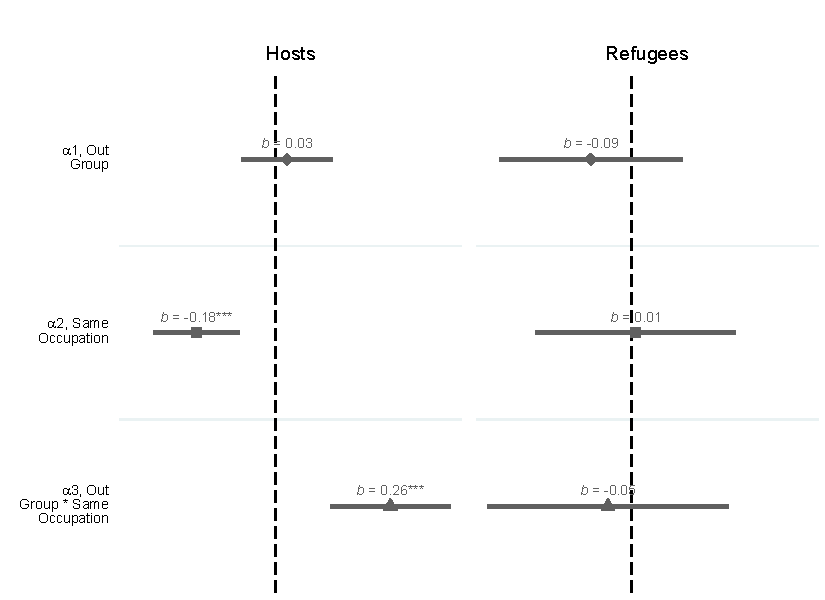
\includegraphics[height=0.4\textwidth]{Figures/FIG4_CFP_Analysis.pdf} \\
        \caption*{
        \footnotesize A positive ($+$) sign means an increase in prejudice. Coefficients b represent changes in standard deviation. An explanation of the coefficients' interpretation can be found in \hyperref[eq:mainspe]{Equation} \ref{eq:mainspe}. We report the Anderson \textit{sharpened False Discovery Rate (FDR) q-values} \cite{anderson2008multiple}, applied over each group individually. Detailed results are presented in Table \ref{tab:main_pooled}. Sample: $n$ = 2,967 for hosts and $n$ = 1,749 for refugees. Weighted regressions. We use the Anderson (2008) index. Standard errors clustered at the PSU level. Significance levels: * p $<$ 0.1, ** p $<$ 0.05, *** p $<$ 0.01. All models include the same control variables. Controls include age, gender, household size, education, and employment status, country of residence, and urban/rural areas.}
        
    \vspace{5mm}
    \end{figure} 

    Partial effects analysis suggests that among hosts, attitudes towards out-group members are more negative than attitudes towards in-group members (Table \ref{tab:main_pooled}), which aligns with expectations under H1. But it is clear that the supportive finding for H1 is driven by negative reactions to out-group members in the same occupation as the host respondent ($\alpha_{3}$). We do not find support of H2 among hosts (Table \ref{tab:main_pooled}), as we measure no significant difference in host self-reported attitudes towards vignette characters in the same occupation overall. However, this insignificant pooled result is overshadowed by contrasting effects: sharing the same occupation with an out-group member leads to an increase in prejudice, while sharing the same occupation with an in-group member results in a decrease in prejudice.
    

For the pooled results for refugees, we do not find statistically significant effects across the variables of interest. It is important to note that the sample size for refugees is smaller than that of hosts. We estimated the minimum detectable size (MDS) for the pooled refugee sample as 0.15 standard deviations (Table \ref{tab:powercalculations}). But even if a larger refugee sample yielded statistically significant coefficients, the results would likely lack economic significance, given the small magnitude of the point estimates.  Our results therefore suggest that the refugee sample viewed the character the same regardless of their identity group or occupation.

We consider our results with clustered standard errors as a conservative approach. To ensure that we may not be overlooking results that are significant without clustering, we estimate our main specifications without any standard error adjustments (Table \ref{tab:nses}). Applying a less conservative approach to standard error estimation, our results remain unchanged.

The main findings, depicted in \hyperref[fig:mainpooled]{Figure} \ref{fig:mainpooled}, rely on the pooled Anderson index, which captures the overall prejudice level across all six attitude questions. To test the robustness of these findings, we modify the construction of the dependent variable by examining potential variations in attitudes across the three different spheres of interaction. The individual results based on indices disaggregated into social and private interactions align with our pooled results (Table \ref{tab:main_disagg}). When we use an index based on work interactions only, all coefficients of interest are null. These insignificant findings may be due to the relatively neutral framing of the attitudes questions around work, which ask the respondent if they ``can'' work with or for the vignette character. The question about whether the respondent ``can work with'' the character also does not impose any working relationship between the respondent and the character. Working at the same firm as an out-group member in the same job may be less salient for respondents if they assume that existing power structures will govern their relationship at work \citep{allport1954nature}.

Results also hold when the dependent variable is transformed into a binary indicator in which 1 is equal to a high level of prejudice: these findings are shown in Table \ref{tab:main_disagg_dummy}. 
Our experiment used desired jobs for the occupations of unemployed respondents (see Appendix Section \ref{annex: unemp analysis}).  It is important that we ensure that our results are not driven by idiosyncratic or strategic responses among those not currently working, but seeking work.  We therefore estimate our main specification separately for those employed and unemployed. The results in (Table \ref{tab:het_emp}) indicate that our main findings hold when we restrict the sample to those who are employed.  

Is the mediating effect of labor market perception restricted to certain types of respondents? Our pooled results do not vary by respondent gender but differ by respondent education (Table \ref{tab:het_2_pooled}). While  $\alpha_{3}$ is statistically zero among hosts with less than primary education, for hosts with primary education or higher, exposure to a character who is a refugee in the same occupation results in a 0.23 standard deviation increase in unfavorable attitudes. Interestingly, refugees with lower levels of education seem more willing to interact with hosts than with other refugees ($\alpha_{1} = -0.33$ for refugees with less than primary education).


\subsection*{Heterogeneity by locality}

The regional analysis in \hyperref[fig:mainpooledbyLoc]{Figure} \ref{fig:mainpooledbyLoc} (details in Appendix Section \ref{annex:het_locality}) provides evidence of stronger out-group prejudice among hosts in urban Addis Ababa, Ethiopia, and rural Isingiro/Nakivale, Uganda, although the underlying mechanisms differ between the two regions.

\begin{figure*}[h]
    \centering
    \captionsetup{width=.7\linewidth}
    \caption{Results by locality}
    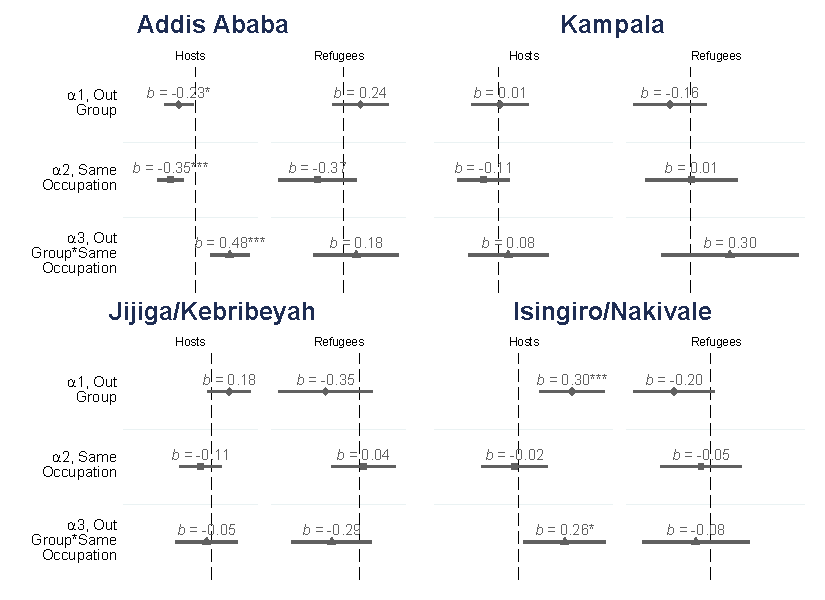
\includegraphics[width=0.7\textwidth]{Figures/FIG5_CFP_Analysis_byLocalities.pdf}
    \label{fig:mainpooledbyLoc}
 \caption*{
 \footnotesize
 The figure includes four panels, each showing results to one of our four locations. A positive ($+$) sign means an increase in prejudice. Coefficients b represent changes in standard deviation. An explanation of the coefficients' interpretation can be found in \hyperref[eq:mainspe]{Equation} \ref{eq:mainspe}. Detailed results are presented in Table \ref{tab:prej_byLoc}. Sample: $n$ = 848 for hosts and $n$ = 198 for refugees in Addis Ababa ; $n$ = 570 for hosts and $n$ = 301 for refugees in Jijiga/Kebribeyah ; $n$ = 691 for hosts and $n$ = 545 for refugees in Kampala ; $n$ = 858 for hosts and $n$ = 705 for refugees in Isingiro/Nakivale. Weighted regressions. We use the Anderson (2008) index. Standard errors clustered at the PSU level. Significance levels: * p $<$ 0.1, ** p $<$ 0.05, *** p $<$ 0.01. All models include the same control variables. Controls include age, gender, household size, education, and employment status, country of residence, and urban/rural areas.}

 \vspace{5mm}
 
\end{figure*}

In Addis Ababa, we estimate a marginally significant (10\% level) and negative $\alpha_{1}$, suggesting less negative attitudes towards refugees in the absence of shared occupational status. Moreover, $\alpha_{2}$ is negative and significant, alluding perhaps to a sense of worker camaraderie among hosts sharing the same occupation. But despite these relatively prosocial views for refugees in different occupations and Ethiopians in the same occupation, attitudes are significantly less open towards a refugee vignette character when they work in the same occupation. Our estimated $\alpha_{3}$ in Addis Ababa is a significant $0.48$ standard deviation increase, reflecting more adverse attitudes when perceived labor market competition is high.

In Isingiro/Nakivale, our research provides evidence of generally negative host views towards refugees, regardless of the occupation of the refugee character in the vignette. ($\alpha_{1}$ is significant and shows a $0.3$ standard deviation increase in the prejudice index). As shown in \hyperref[tab:regression_comparisons]{Table} \ref{tab:regression_comparisons}, the estimated coefficient at 0.3 is statistically different from the equivalent coefficient for Addis Ababa ($-0.23$). The $\alpha_{3}$ estimate is positive, but is smaller in magnitude ($0.26$) than our finding in Addis Ababa and only weakly significant at the 10\% level. Post estimation testing recovers no significant difference between the $\alpha_{3}$ coefficients estimated in Addis Ababa and Nakivale/Isingiro. This null result may relate to the lack of precision and wider standard errors on the $\alpha_{3}$ finding for Nakivale/Isingiro. No significant differences in attitudes across treated groups could be observed in the two remaining sites, Kampala (Uganda) and Jijiga/Kebribeyah (Ethiopia). 


As in the pooled results, we find little evidence that refugees hold different attitudes towards the vignette character when we modify its group membership (refugee/ host) or occupation (same/ different). However, we cannot reject the possibility that null results for refugees are partly due to small sample sizes (\hyperref[tab:powercalculations]{Table} \ref{tab:powercalculations}). For example, our survey only captured 198 refugees in Addis Ababa, and with this sample size, the locality regression may be underpowered.



\section{Discussion}


The results of our experiment support the argument that host community members hold prejudicial views of refugees when perceived labor market competition is high. Our heterogeneity analysis reveals important differences across study locations, highlighting the importance of contextual background in shaping attitudes towards refugees. 

Our pooled result on out-group prejudice towards a fictitious refugee character described as having the same occupation is stronger for Ethiopian respondents in Addis Ababa. Among the four study sites of our analysis, Addis Ababa is unique in its recent receipt of conflict-driven inflows of Eritrean refugees from Tigray to the capital \citep{tsegay2023internal}. As mentioned earlier, the refugee population in Addis Ababa doubled between January 2021 and July 2022 \citep{ethiopiaStatsNov22}. Our findings may speak to growing concerns over job competition in Addis Ababa due to the internal displacement of refugees who are eligible to work \citep{miller2021}. But even with this population increase, refugees in Addis Ababa represent a very small fraction of the city's population (only 1.2\% as of 2022). Consequently, we posit that our findings are more likely attributable to perceptions of competition that do not fully align with reality. In this case, the salience of our finding manifesting in Addis Ababa echoes a past observation from \cite{allport1954nature}: prejudice against out-groups intensifies during periods of duress and during periods in which the out-group's population is growing. 

For Isingiro/ Nakivale, we find evidence of negative attitudes towards refugees that are independent of private labor market concerns. Relative to other sites, a large share of the Isingiro/Nakivale population consists of refugees. Additionally, Uganda's self-reliance refugee policy emphasizes sharing resources with hosts and integration of refugees into markets. Hence, the feeling of competition for resources might play a role in enhancing generalized out-group antagonism. For instance, \citet{betts2023refugees} show that villagers in Nakivale view refugees as a threat to their livelihoods because they rely on farming and animal husbandry, and refugees also participate in these livelihoods activities. Hence, hosts may not perceive refugees as competitors for wage employment, but may see refugees as a source of competition in terms of agricultural inputs such as land.  Our results, therefore, echo recent publications that stress the limits of inclusive services and refugee self-reliance policies in fostering societal harmony \citep{omata2022rethinking}. If hosts believe that refugee hosting constitutes a net loss (despite the inflow of benefits received as part of inclusive services), this could shape hosts' broader perceptions of refugees.

We cannot formally test for the role of different political, social and cultural contexts in shaping out-group attitudes across our four study sites, given limitations on statistical power. However, we are able to identify potential mechanisms of increased out-group prejudice by focusing on individual-level heterogeneitiy in our pooled sample. The contrasting results between Addis Ababa and Isingiro/Nakivale suggest that misconceptions of refugees as job competitors - rather than any realized labor market competition -  may serve as a primary drivers of prejudicial attitudes towards refugees working in the same job as hosts. To further examine this possibility at the individual level, we examine heterogeneity by labor market competitiveness from the perspective of workers, proxied by the share of respondents in a given industry-location who work more than the legal maximum of 48 hours per week. We consider labor hours exceeding the legal maximum as a signal of particularly competitive local labor market where vacancy rates are low and consequently wages are low, increasing the incentive to work more hours per week. 


	\setstretch{1}
\begin{table}[H]
	\footnotesize
	\caption{Summary Table: Refugee-Host relationships}
	\label{Summary}
	\centering
	\begin{threeparttable}
			\begin{tabular}{l*{4}{l}} \toprule 
                &\multicolumn{2}{c}{(1)}&\multicolumn{2}{c}{(2)}\\
                &\multicolumn{2}{c}{ } &\multicolumn{2}{c}{ } \\
\\[-0.6cm] & \multicolumn{4}{c}{\textit{Hosts as respondents}}  \\ \midrule \multicolumn{5}{c}{\textbf{PANEL A: Working hours beyond legal threshold}} \\ & \multicolumn{2}{c}{\textit{High share over-worked}} & \multicolumn{2}{c}{\textit{Low share over-worked}}   \\  \midrule  
$\alpha1$: OutGroup (1) vs InGroup (0)&    -0.12   &   (0.10)&     0.14*  &   (0.08)\\
$\alpha2$: Same (1) vs Different (0) Occupation&    -0.31***&   (0.08)&    -0.08   &   (0.08)\\
 
$\alpha3$: OutGroup x Same Occupation&     0.39***&   (0.12)&     0.16   &   (0.11)\\
 
H1: OutGroup (1) vs InGroup (0)&     0.08   &   (0.07)&     0.21***&   (0.06)\\
 
H2: Same (1) vs Different (0) Occupation&    -0.11*  &   (0.06)&    -0.01   &   (0.06)\\
 
  \\\\[-0.5cm] N \\\\[-0.6cm]&     1321   &         &     1644   &         \\
Mean            &     0.01&         &     0.02&         \\
 
 \\ \midrule \multicolumn{5}{c}{\textbf{PANEL B: Over-representation by industry}} \\ & \multicolumn{2}{c}{\textit{Hosts overrepresented}} & \multicolumn{2}{c}{\textit{Refugees overrepresented}}   \\  \midrule  
$\alpha1$: OutGroup (1) vs InGroup (0)&     0.07   &   (0.08)&    -0.02   &   (0.11)\\
$\alpha2$: Same (1) vs Different (0) Occupation&    -0.16** &   (0.07)&    -0.21** &   (0.10)\\
 
$\alpha3$: OutGroup x Same Occupation&     0.29***&   (0.10)&     0.10   &   (0.15)\\
 
H1: OutGroup (1) vs InGroup (0)&     0.22***&   (0.05)&     0.03   &   (0.09)\\
 
H2: Same (1) vs Different (0) Occupation&    -0.02   &   (0.05)&    -0.16*  &   (0.09)\\
 
  \\\\[-0.5cm] N \\\\[-0.6cm]&     2076   &         &      751   &         \\
Mean            &     0.02&         &     0.02&         \\
 
 \\ \midrule \multicolumn{5}{c}{\textbf{PANEL C: Contact}} \\ & \multicolumn{2}{c}{\textit{No out-group friends}} & \multicolumn{2}{c}{\textit{Some out-group friends}}   \\  \midrule  
$\alpha1$: OutGroup (1) vs InGroup (0)&     0.04   &   (0.07)&     0.02   &   (0.11)\\
$\alpha2$: Same (1) vs Different (0) Occupation&    -0.19***&   (0.07)&    -0.15   &   (0.13)\\
 
$\alpha3$: OutGroup x Same Occupation&     0.31***&   (0.10)&     0.09   &   (0.15)\\
 
H1: OutGroup (1) vs InGroup (0)&     0.20***&   (0.05)&     0.07   &   (0.08)\\
 
H2: Same (1) vs Different (0) Occupation&    -0.04   &   (0.05)&    -0.11   &   (0.08)\\
 
  \\\\[-0.5cm] N \\\\[-0.6cm]&     2227   &         &      740   &         \\
Mean            &     0.02&         &     0.01&         \\
 
 \\ \midrule \multicolumn{5}{c}{\textbf{PANEL D: Out-group language}} \\ & \multicolumn{2}{c}{\textit{Different language}} & \multicolumn{2}{c}{\textit{Shared language}}   \\  & \multicolumn{2}{c}{\textit{(main out-group language)}} & \multicolumn{2}{c}{\textit{(main out-group language)}}  \\ \midrule  
$\alpha1$: OutGroup (1) vs InGroup (0)&     0.02   &   (0.07)&     0.08   &   (0.14)\\
$\alpha2$: Same (1) vs Different (0) Occupation&    -0.18***&   (0.07)&    -0.15   &   (0.15)\\
 
$\alpha3$: OutGroup x Same Occupation&     0.31***&   (0.09)&     0.01   &   (0.20)\\
 
H1: OutGroup (1) vs InGroup (0)&     0.18***&   (0.05)&     0.09   &   (0.09)\\
 
H2: Same (1) vs Different (0) Occupation&    -0.03   &   (0.05)&    -0.15   &   (0.11)\\
 
  \\\\[-0.5cm] N \\\\[-0.6cm]&     2468   &         &      499   &         \\
Mean            &     0.03&         &    -0.05&         \\
 
\bottomrule  \end{tabular}  

		\begin{tablenotes}
	\footnotesize
	\item Weighted regressions. We use the Anderson (2008) index. Standard errors clustered at the PSU level. Significance levels: * p $<$ 0.1, ** p $<$ 0.05, *** p $<$ 0.01. All the models include the same control variables. Controls include age, gender, household size, education, employment, country of residence, and urban/rural areas. The sample is stratified according to the percentage of respondents reporting weekly working hours exceeding the legal threshold of 48 hours. Panel A consists of respondents employed in industry-location groups where the percentage of individuals working beyond the legal limit exceeds (falls below in column 2) the median share. The median share of such workers across all industries in the four different localities stands at 56\%. Detailed results -- including when the respondent is a refugee -- are presented in Appendix  \hyperref[tab:comp_hi_lo]{Table} \ref{tab:comp_hi_lo}.  In Panel B (hosts or refugees over-represented), we include respondents working in industries where the proportion of hosts (refugees) exceeds the local average. Detailed results are presented in Appendix  \hyperref[tab:het_repres]{Table} \ref{tab:het_repres}. In Panel C, the 5-scale source question -\textit{Over the course of my life, I have had many friends who are [Ugandan/Ethiopian nationals]/[Refugees]}, respectively- was transformed into a binary with the unit agreeing with the statement, and the null disagreeing or being neutral. Detailed results are presented in Appendix Table \ref{tab:contact}. Panel D comprises respondents with a distinct ethno-linguistic identity compared to the other group. The criteria for this distinction are defined independently for each locality, taking into account the predominant language spoken by the out-group. Detailed results are presented in Appendix Table \ref{tab:het_ethno}.
\end{tablenotes}
\end{threeparttable}
\end{table} 
\vspace{8mm}
\setstretch{1}

\onehalfspacing As summarized in Panel A of Table \ref{Summary}, we find that the mediating role of perceived labor market competition in triggering out-group prejudice is stronger in sectors with competitive labor markets, as proxied by excessive working hours (see Appendix \hyperref[tab:comp_hi_lo]{Table} \ref{tab:comp_hi_lo} for full results). Interestingly, hosts in such competitive labor markets report significantly more \textit{positive} views of an in-group vignette character working in the same occupation ($\alpha_2$). The significant and positive finding for $\alpha_3$ and significant, negative result for $\alpha_2$ among hosts in competitive labor markets may mean that respondents in industry-locations with high competition among workers are concerned about this competition, but only when the source of the competition is perceived as the refugee population.

We further explore the practical basis of prejudice-aligned perceptions of job competition by examining the heterogeneity of our results by refugee worker presence. Specifically, we identify whether the pool of workers in a respondent's industry-location have a higher share of hosts than the location's average share across all workers. Negative attitudes towards a perceived job competitor may be based on experience or observation if these attitudes manifest among host respondents who work alongside many refugees. But negative attitudes among workers in industry-locations with low refugee representation suggest that the prejudice is not aligned with the genuine situation of the labor market. As summarized in Panel B of Table \ref{Summary}, we find that in industry-locations where hosts are over-represented relative to the location's average, host attitudes towards a refugee vignette character sharing the same occupation are more antagonistic. We find no evidence of prejudicial attitudes  among host respondents working in industries where hosts are not over-represented (see Table \ref{tab:het_repres} for detailed results). This finding suggests that host prejudice towards refugees working in the same occupation manifests among hosts who face the least competition with refugees in the labor market. It is possible that host respondents in competitive labor markets correctly identify labor market competition as a salient concern but may mistakenly blame refugees for this competition. In these contexts, refugees may serve as a scapegoat for societal concerns. This possibility aligns with past work highlighting how societies assign blame to refugees for social or economic problems \citep{baylouny2020, savun2019protection, hanson2010out}.


Contrasting results across studied sites also suggest that the mediating role of perceived labor market competition is not determined by the numbers of refugees, but by the nature of refugee-host relationships. This qualification is further supported when the sample is stratified by respondents indicating whether or not they have at least one friend who is a member of their out-group. For hosts, this would mean having at least one friend who is a refugee. Panel C of Table \ref{Summary} (and Table \ref{tab:contact}) suggests that hosts with limited refugee contact are driving the significant main result for $\alpha_{3}$. Although prior contact may be endogenous to other factors, this additional analysis may suggest that addressing prejudicial attitudes could be aided by interventions that increase inter-group contact. In the absence of strong adversarial inter-group contact \citep{lowe2021}, we conjecture that out-group contact facilitates perspective-updating which likely results in reduced perception of competition. 

When the respondent is a refugee, the results by locality are either not statistically significant or are more likely to go in the opposite direction. It is unclear whether this represents refugee enthusiasm for building local ties with hosts or refugee antagonism toward other refugees. We recognize that refugee respondents may still interpret a refugee vignette character as an out-group member if they imagine that the character is of a different nationality as their own. Past literature points out that not all refugee communities within the same hosting areas get along \citep{bjorkhaug2020revisiting}. Among refugees, contact also seems to matter for the outcomes of the experiment. In particular, the refugee respondents' prejudice index is on average $0.37$ standard deviation lower towards a host character relative to a refugee character ($\alpha_{1}$) (Table \ref{tab:contact}). 

The differing results across study sites may also be explained by variations in ethnolinguistic proximity. In their quasi-experimental evidence on social cohesion in Ethiopia, Kenya and Uganda, \citet{betts2023refugees} find that ethno-linguistic proximity between refugees and hosts is associated with more positive host attitudes towards refugees. Recently, scholars have also argued that the ethnic and/or cultural proximity of Ukrainians and European host countries explains the supportive hosting policies and positive public reception that displaced Ukrainians received in 2022 
 \citep{leonard2022europe, bosilj2022european}.  According to \citet{de2023refugee} and \citet{iordache2024perceptions}, the European public's disparate perceptions towards Ukrainian and Afghan refugees is largely attributable to ethnic proximity and distance.

 The spatial heterogeneity of our sample leads to differences in the ethno-linguistic similarity of refugee and host groups across the four study sites. While refugees and hosts in the Jijiga/ Kebribeyah area mainly share the same language and ethnicity (Somali), the ethno-linguistic composition in the other study contexts is more diverse. Turning to an individual-level heterogeneity analysis, we find that prejudice towards refugees is exclusively driven by those respondents who do not share the ethno-linguistic characteristics of the refugees within the same locality (Panel D of Table \ref{Summary} and Table \ref{tab:het_ethno}). This supports the argument that ethno-linguistic proximity could be partially explaining the prejudice of hosts towards refugees in Addis Ababa (Ethiopia) and Isingiro/Nakivale (Uganda). This finding aligns with and supports the past findings that ethno-linguistic proximity facilitates a sense of community, lowering the likelihood of prejudice against refugees \citep{de2023refugee, betts2023refugees, hynie2016social}. Prejudice also appears to be smaller when the respondent is part of an ethno-linguistic minority group, indicating possible empathy towards the out-group (Table \ref{tab:het_major}).


\section{Conclusion}

\noindent Fostering refugee inclusion is critical for improving refugee livelihoods in cases of protracted displacement. Our study examines the role of perceived job market competition on out-group attitudes in refugee hosting settings in East Africa. Our vignette experiment seeks to stimulate realistic reactions to a fictional character whose profile is identical across all respondents, with the exception of two attributes: we randomize whether the character is a refugee or host, and we randomize whether the character works in the same occupation as the respondent or in a different occupation requiring a similar education level as the respondent's. After exposure to our vignette, respondents self-report their attitudes towards the character within the context of their private, social, and working life. We exploit the random assignment of the character's occupation and citizenship status to estimate differences in self-reported attitudes operationalized within an Anderson Index.

Our pooled results suggest that host attitudes towards refugees are largely mediated by perceived job market competition, as proxied by the vignette character working in the same job as the respondent. But heterogeneity analysis by locality reveals that these results are largely driven by host respondents in Addis Ababa. 

Given variation in outcomes by localities of different attributes, we explore heterogeneity by labor market characteristics. Our results suggest that host respondents hold more negative attitudes towards refugees working in the same occupation in labor markets characterized by high competition among workers and low refugee representation. This finding implies that hosts may have a salient concern over job competition. But importantly, the concentration of prejudicial attitudes tied to perceived job competition among those who face very little competition with refugees suggests that hosts may be incorrectly associating refugees with job competition. According to \cite{allport1954nature}, such unsubstantiated beliefs about outgroup members may be more likely in social contexts characterized by sudden change and increases in the outgroup population, as in the case of Addis Ababa. Such misattribution may also be more likely in cases where host workers have less contact with refugees. 

Furthermore, ethnolinguistic distance or the lack of inter-group contact may also explain some of the prejudice of hosts against the refugees. The contact result may reflect endogenous individual preferences, but could also reflect the value in repeated exchange in addressing incorrect priors about outgroups.

Our work suggests that unsubstantiated beliefs of refugees as a threat to livelihoods worsens perceptions of refugees among hosts, weakening the prospect of social inclusion. The findings suggest that improving refugee-host relationships does not require policies that shield host workers from (non-realized) refugee job competition, such as prohibiting refugees from working or limiting the sectors they can work in. Instead, policymakers must consider socially-oriented interventions. Informational campaigns may help address incomplete information about refugees and the labor market. But such efforts must be socially widespread, as informational interventions that target individual in-group members may fail in the long run because the ingroup's shared beliefs concerning the outgroup may overpower any new information \citep{allport1954nature}. Our results related to contact suggest that inter-group interaction may also address negative attitudes towards refugees. Such efforts may be more successful within a policy design in which the two groups work together towards a common goal \citep{barros2023power}.

Our study is not without limitations. In particular, our findings may not be externally valid to other refugee-hosting countries or contexts. With only four case study settings, it is difficult to reliably determine the mechanisms that influence variation in attitudes and the mediating role of perceived labor market perception across the study sites. For example, in Addis Ababa, we do not know if the negative host reactions to the refugee vignette character working in the same job are indirectly related to the Tigray War and whether we would find the same result at times of peace. We encourage future efforts that seek to understand the factors that influence in-group and out-group attitudes in refugee hosting settings, considering the role of labor market competition. More work needs to be done to understand the triggers of perceived labor market competition among hosts. And importantly, we encourage future work that develops methods to foster refugee integration by addressing negative and unsubstantiated priors among host communities. 
\pagebreak

\singlespacing
%\section{Bibliography}

%
% ---- Bibliography ----
%
% BibTeX users should specify bibliography style 'splncs04'.
% References will then be sorted and formatted in the correct style.
%
%\bibliographystyle{aea}
\bibliography{Bibliography.bib}
%
\clearpage

%TC:ignore

\makeatletter
\renewcommand{\thefigure}{A\@arabic\c@figure}
\renewcommand{\theequation}{A\@arabic\c@equation}
\renewcommand{\thetable}{A\@arabic\c@table}
\renewcommand{\thesection}{A\arabic{section}}
\makeatletter
\renewcommand{\figurename}{Figure}
\renewcommand{\tablename}{Table}
\renewcommand{\baselinestretch}{1}
\setcounter{section}{0}
\setcounter{figure}{0}
\setcounter{equation}{0}
\setcounter{table}{0}

%\begin{center}
%    \textbf{Supplemental Online Appendix}
%\end{center}

	%\pagebreak
	
%%%%% APPENDIX


	
	\begin{appendix}

%\appendix 



\onehalfspacing

\section{Appendix}


\subsection{Deviation from the Pre-Analysis Plan (PAP)} \label{A1 Dev from PAP}

\noindent \hyperref[tab:deviation]{Tables} \ref{tab:deviation} and \ref{tab:addition} provide a summary of deviations from the PAP, encompassing both supplementary analyses that were not pre-registered and adjustments or omissions of exclusions initially specified in the study.  These deviations are not motivated by the magnitude or statistical significance of the estimated coefficients, but by methodological improvements, conceptual clarifications or unexpected practical challenges.\\


%ADD : WE REMOVE MARITAL STATUS FROM CONTROL VAR

%ADD : "If power allows, we will also test to which extent previous interactions with the out-group (contact hypothesis) and reported competition on the labor market (subjective measure) as well as de facto competition on the local labor market (objective measure: density of different occupations within host and refugee groups) link back to our results."

\singlespacing

\begin{longtable}[c]{m{8em}m{12cm}}
    \caption{Deviation from the PAP} 
    \label{tab:deviation} \\
    \hline
    \textbf{Exclusions} & \textbf{Explanation} \\
    \hline\hline
    \endfirsthead
    \hline
    \textbf{Exclusions} & \textbf{Explanation} \\
    \hline\hline
    \endhead
    \multicolumn{2}{r}{Continued on next page} \\
    \endfoot
    \endlastfoot
    The term ``discrimination'' & In the PAP, particularly when formulating our hypotheses for testing, we use the term ``discrimination.'' For example, we state, ``\textit{H3: Discrimination against members of the out-group is more pronounced when preconceived notions of labor market competition are strong}''. We have replaced this term with ``prejudice,'' which conveys self-reported attitudes, as the term ``discrimination'' implies that we would be evaluating revealed preferences through observed actions or measuring psychometrics, which is not within the scope of our study. \\
    \hline
    Target sample size & We aimed to have a total sample of 8,000 households, comprising 4,000 host community members (nationals) and 4,000 refugees, both employed and unemployed, distributed between rural and urban areas in Uganda and Ethiopia. Due to difficulties to locate refugee households (especially in urban areas), low response rates and logistical and budget constraints, the target sample size could not be reached for all sub-groups (see \hyperref[tab:sampledescexp]{Table} \ref{tab:sampledescexp}). Further reduction occurred during the third sampling stage, where individuals were randomly selected to participate in the experiment, limited by age constraints (only respondents of working age were included). As outlined in \hyperref[sec:Sampling and data collection]{Section} \ref{sec:Sampling and data collection} above, this adjustment in sample size did not impact the implementation of our experiment because randomization was carried out at the individual level. For some heterogeneous analyses for the group of refugees, smaller sample size is however limiting statistical power of our analysis. \\
    \hline    
    Reporting the \textbf{\textit{H1}} \& \textbf{\textit{H2}} regression coefficients & According to the PAP, we are testing 3 hypotheses; \textbf{\textit{H1}}, \textbf{\textit{H2}} \& \textbf{\textit{H3}} with the following regression.
    \begin{equation} 
        \label{eq:mainspe}
        \begin{split}
            y_{i} = \alpha_{0} + \alpha_{1} OutGroup_{i} + \alpha_{2} SameOcc_{i} \\
            + \alpha_{3} (OutGroup_{i} * SameOcc_{i}) + X_{i}^{'} \gamma + u_{i}
        \end{split}
    \end{equation} 
    The answer to Hypothesis \textbf{\textit{H3}} is derived from $\alpha_{3}$ in our long model (1). However, \textbf{\textit{H1}} \& \textbf{\textit{H2}} could in principle be answered with a ``short model'', which involves regressing the dependent variable on two separate dummies for both treatments. The partial effects of this fully saturated long model are equivalent to the coefficients of the short model, so we refrain from reporting separate regressions. On the one hand, $\alpha_{1}$ represents the coefficient of prejudice for those who see the vignette of an out-group but with different occupation and $\alpha_{2}$ represents the coefficient of prejudice for those who see the vignette of a character with same occupation but belonging to the in-group. On the other hand, \textit{H1} represents the coefficient of prejudice for those who see the vignette of an out-group irrespective of the occupation characteristic and \textit{H2} represents the coefficient of prejudice for those who see the vignette of a character with same occupation irrespective of belonging to the out-group or in-group. When providing answers to our hypotheses (1 \& 2), we always interpret the \textit{H} coefficients together with the underlying $\alpha$ coefficients. Contrary to the PAP, we do not only report our \textit{H} coefficients, because from a political perspective, we would not have a similar distribution in the general household sample as in the experimental sample. Therefore, the underlying $\alpha$ coefficients are what are truly important. Hence, we present the $\alpha$ coefficients in the figures within the main text and infer all estimates for the three hypotheses from the long model, reporting marginal effects as \textit{H1} \& \textit{H2} coefficients in the \hyperref[tab:main_pooled]{Tables} \ref{tab:main_pooled} and \ref{tab:prej_byLoc}  in \hyperref[annex:mainresults]{Annex} \ref{annex:mainresults}. \\
    \hline
    Heterogeneity by key occupational characteristics & We intended to examine the relative effect of being categorized by occupation, for instance as either employers, own account workers, or wage workers, on attitudes. Whilst the analysis, split between self-employed workers and wage workers (available upon request) leads to some new results on the group of refugees, the sample distribution does not offer enough variation or large enough sample size to avoid significant concerns with statistical power.\\
    \hline
    Analysis on the entire outgroup & In the PAP, we planned to examine whether our treatment had an impact on prejudice towards a generalized out-group, independently of the fictitious character.  We thus included a set of questions measuring private and work-related prejudice that was not framed for Aida/ Robert, but for the out-group overall. These questions were administered in the module following the experiment and relate to both nationals and refugees (i.e., a refugee would answer a question related to a host, and vice versa). We do not observe any differences in results between Panel A and B, both at the aggregated and individual-variable levels. However, we initially intended to mirror our experimental setting, i.e., let all individuals also answer the questions on the ``in group''. Because of field constraints, we couldn't implement this setup during our data collection. We henceforth decided not to show the analysis in the paper, albeit the partial results are available upon request. \\
    \hline
    Marital status as covariate & We exclude marital status from the list of covariates in the regressions. As this variable contains missing observations, including it as a control variable in the regressions reduces the final sample size by 11 observations. This drop in sample count is only observed with the inclusion of marital status as a covariate and not with the other covariates. None-the-less, excluding marital status as a control does not bias our coefficients of interest $\alpha_1$, $\alpha_2$ and $\alpha_3$ since we find, from the balance tests, that the treatment group assignment is also balanced along the respondents' marital status.\\
    \hline
\end{longtable}

\vspace{5mm}
      \begin{table}[H]
        \begin{center}
        \caption{Addition to the PAP}
        \label{tab:addition}
               \begin{tabular}{m{8em}m{12cm}}
                \hline
                 \textbf{Additional Analysis} & \textbf{Explanation} \\
                \hline\hline
                & \\[-0.8em]
 Heterogenous analyses by locality, gender, education level, \& ethno-linguistic proximity. & Anticipating statistical power constraints, the initial plan was to divide the analysis by country to explore the potential impact of differing refugee management approaches in Ethiopia and Uganda. However, we discovered that it would be meaningful to further conduct a split analysis by locality. This is because of the substantial differences in local characteristics, particularly the possible contextual differences between the urban and rural settings, which could interact in various ways with the policy environments in the countries and result in
varying responses among the study participants. Additionally, since we assigned respondents to view a vignette narrative featuring a character of the same gender, we did not consider gender as a treatment variable. This approach allows us to investigate whether the attitudes of males are comparable to those of females within this context. Similarly, we applied this approach to assess the relative importance of education level, which can serve as a proxy for skill level and, consequently, predisposition to certain types of jobs in the market. Furthermore, in alignment with the contact theory, where we examine the significance of having friends from the out-group, we also explore the relevance of ethno-linguistic proximity, which may serve as a mediating variable. \\ 
                \hline
                \end{tabular}
        \end{center}
    \end{table}


\subsection{Sampling and data collection}
\label{sec:Sampling and data collection}

\onehalfspacing

Our study uses a vignette experiment that was embedded in a large survey on refugee-host interactions and labor market integration, designed and commissioned by the World Bank.\footnote{The survey aims at gathering comparable data in four refugee-hosting localities in Uganda and Ethiopia. It collects household-level information on socio-demographic characteristics as well as individual data on labor market characteristics, refugee-host interactions and social networks for one randomly selected individual (RSI) per household. The survey experiment described here is part of the RSI questionnaire.} FAFO, an implementation partner, collected survey responses from late January 2022 to late July 2022 in Uganda and Ethiopia. 
 
The data from the larger survey is described in World Bank (2023). Samples were drawn to represent the refugee population and host populations in two urban and two rural settings. In Ethiopia, data was collected from the city of Addis Ababa as the urban location with 150 EAs. Jijiga (45 EAs) and Kebribeyah, including Kebribeyah refugee settlement, (35 EAs) serve as the rural locations. 
 
The sampling exercise relied on pre-existing sampling frames containing the primary sampling units (PSUs), which correspond to enumeration areas (EAs). In Ethiopia, the Central Statistical Agency provided a sampling frame that was originally intended for use in a planned (but never implemented) 2020 Census. In Uganda, the sampling frame was provided by the Uganda Bureau of Statistics (UBOS). The sampling procedure incorporated modifications to capture sufficient sample sizes for both refugees and hosts. 
 
In the first round of EA selection, the team used a Probability Proportionate to Size (PPS) approach to select the first set of EAs. This first set of EAs contains both host and refugee households. To obtain sufficient numbers of refugee households in the final sample, the study team conducted a second sampling round that selected additional EAs bordering those chosen in the first round of EA selection. For Addis Ababa, where refugee households are difficult to capture using conventional sampling methods, the team used an Adaptive Cluster Sampling strategy (ACS) in which refugee households were identified for sampling.  
    
Following a complete listing of households, the samples were drawn to represent the population of refugees and host populations in two urban and two rural settings. In Ethiopia, data was collected from the city of Addis Ababa as the urban location with 150 AEEs. Jijiga (45 EAs) and Kebribeyah, including Kebribeyah refugee settlement, (35 EAs) serve as the rural locations.\footnote{In the rest of the manuscript, we mention Jijiga/Kebribeyah as the aggregation between Jijiga and Kebribeyah, both considered rural areas.} In Uganda, the rural EAs fall in the Isingiro district (75 EAs) and the Nakivale refugee settlement (40 EAs).\footnote{In the rest of the manuscript, we mention Isingiro/Nakivale as the term that encompasses both the town of Isingiro and the Nakivale settlement, both considered rural areas.} For urban Uganda, the EAs fall in the Kampala district with 150 EAs.\footnote{Our results are representative of host and refugee outlooks in the four study sites examined. The findings may not be externally valid to other refugee-hosting countries or contexts. Throughout, we discuss the exact findings in relation to the experiment, and additional discussion of what these results may convey (in terms of respondent's behaviors) are primarily speculative.} 

In the second stage of the sampling, households were then sampled from the EAs. A third sampling stage was performed to obtain a randomly selected individual (RSI) for the experiment; only one individual per household, of working age (18 – 65 years) irrespective of employment status (employed or unemployed). Field constraints limited our sample sizes in some locations. Our final sample is described in  \hyperref[tab:sampledescexp]{Table} \ref{tab:sampledescexp}. This change in sample size does not affect the rollout of our experiment, since the randomization was performed independently of group size, sampling stratification and at the individual level. \\ 


For the household survey, Addis Ababa had a high (84\%) response rate. Non-response was largely due to no-contacts (10\%), while 4\% of households refused to participate. Among those who completed the household survey, the majority (96\%) completed the randomly selected individual (RSI) questionnaire that our experiment was embedded in. In 4\% of cases, the RSI was not collected from a sample household due to no-contacts (individual not available due to lack of time, or due to an accident or illness), or due to changes in identity between the listing and the survey response \citep{fafo2025}. 
%We believe that the low refugee sample count in Addis Ababa speaks to the difficulty of sampling refugees based on a two-stage procedure prioritizing refugee-dense areas. This approach improves refugee representativeness in the data, but a random sample of households in refugee-dense neighborhoods will still include many non-refugees. 

Our final sample consists of 4,716 individual respondents: 1,749 refugees and 2,967 hosts. Table \ref{tab:sampledescexp} reports sample counts by location and group. \\



\begin{table}[H]
    \begin{center}
    \caption{Study sample}
    \label{tab:sampledescexp}
    \small
        \begin{adjustwidth}{0cm}{}
            \renewcommand{\arraystretch}{2.3}  % Increase row spacing globally
            \begin{tabular}{m{4em}m{5em}m{4cm}m{4cm}m{3cm}}
            \textbf{Country} & \textbf{Residence} & \textbf{Location} & \textbf{Enumeration areas} & \textbf{N} \\
            \hline\hline
            Uganda & Rural & Isingiro District & Isingiro/Nakivale: 94 & \pbox{20cm}{858 hosts,\\[-0.2em] 705 refugees} \\
            Uganda & Urban & \pbox{20cm}{Kampala District} & Kampala: 195 & \pbox{20cm}{691 hosts,\\[-0.2em] 545 refugees} \\[0.5em]  % Add small space between main rows
            Ethiopia & Rural & Somali region & Jijiga/Kebribeyah: 31 & \pbox{20cm}{570 hosts,\\[-0.2em] 301 refugees} \\
            Ethiopia & Urban & Addis Ababa & Addis Ababa: 262 & \pbox{20cm}{848 hosts,\\[-0.2em] 198 refugees} \\
            \end{tabular}
        \end{adjustwidth}
    \end{center}
\end{table}

While the sample was drawn to be representative of the local population, the lower response rate raises the question of whether there is potential selection bias among our respondents. \hyperref[tab:summary_stats]{Table} \ref{tab:summary_stats} demonstrates that the descriptive statistics for HHR-LMS households are largely comparable to those of households interviewed in the same four sub-regions by the nationally representative LSMS surveys (the 2021/2022 Socio-Economic Panel Survey for Ethiopia (ESPS) and the 2019/2020 Uganda National Panel Survey (UNPS)). Despite slight differences in both time (as our data was collected in 2022, compared to the 2019/2020 UNPS and 2021/2022 ESPS) and space (as the LSMS analysis is limited to the sub-regions in which our study sites are located), we still find that the descriptive statistics are largely comparable.

\vspace{5mm}

\begin{table}[ht]
	\centering
	\begin{threeparttable}
		\caption{Summary Statistics: HHR-LMS vs LSMS}
		\label{tab:summary_stats}
		\scriptsize
		\begin{tabular}{lcccccc} \toprule
\textbf{Panel A: Ethiopia} & \multicolumn{3}{c}{\textbf{HHR-LMS}} & \multicolumn{3}{c}{\textbf{LSMS}} \\
\cmidrule(lr){2-4} \cmidrule(lr){5-7}
& \textbf{Mean} & \textbf{SD} & \textbf{Obs} & \textbf{Mean} & \textbf{SD} & \textbf{Obs} \\ \midrule
\midrule
Male                &        0.52&        0.50&        1418&        0.51&        0.50&        3504\\
Age of the respondent&       32.81&        9.98&        1418&       35.26&       11.94&        3504\\
Received at least primary education&        0.63&        0.48&        1418&        0.47&        0.50&        3080\\



Household Size      &        5.10&        2.59&        1418&        5.61&        2.50&        1147\\
\bottomrule  \end{tabular}  
\begin{tabular}{lcccccc} 
\textbf{Panel B: Uganda} & \multicolumn{3}{c}{\textbf{HHR-LMS}} & \multicolumn{3}{c}{\textbf{LSMS}} \\
\cmidrule(lr){2-4} \cmidrule(lr){5-7}

Male                &        0.40&        0.49&        1549&        0.50&        0.50&        1037\\
Age of the respondent&       34.33&       11.20&        1549&       34.25&       12.37&        1037\\
Received at least primary education&        0.66&        0.47&        1549&        0.72&        0.45&        1025\\



Household Size      &        4.57&        2.48&        1549&        4.47&        2.57&         435\\
\bottomrule  \end{tabular}  

		\begin{tablenotes}
			\footnotesize
			\item \textit{Notes:} We use sampling weights for all datasets. HHR-LMS descriptive statistics are based on the Randomly Selected Individual (RSI) sample used for the analysis in this paper. LSMS data stems from the ``Socio-Economic Panel Survey 2021–2022'' for Ethiopia and the ``Uganda National Panel Survey 2019–2020'' for Uganda. For both countries, the LSMS data is restricted to the regions included in this analysis: Addis Ababa and the Somali region for Ethiopia, and Kampala and Ankole for Uganda. Additionally, the LSMS analysis is limited to individuals in the labor force (aged 18–65 years), consistent with the RSI sample of the HHR-LMS survey.
		\end{tablenotes}
	\end{threeparttable}
\end{table}



\subsection{Additional information on the experiment} \label{sec: additional experiment}

We implement the survey experiment with all respondents who are currently employed or unemployed: respondents out of the labor force are excluded from the experiment. For each respondent, we randomize the vignette character's citizenship status as being a national or a refugee, meaning that refugee and host respondents alike are randomly exposed to a story about an in-group or out-group member. We use information from the labor module to determine the respondent's primary occupation, and we randomly set the vignette character's occupation to be the same as or different than the respondent's. When interviewing respondents who are unemployed at the time of the interview, we inquire about their preferred occupation in the labor module and incorporate this desired occupation within the vignette. We designed the randomization such that when matching to vignette characters with a different occupation. The vignette character's occupation is at the same skill level as the respondent. For example, a respondent who is a farmer may be matched with a respondent who is a waiter or cleaner.The rationale for restricting the definition of a different occupation within the same skill set was to avoid priming differences in social class or status of the different occupation.

We use information from the labor module to determine the respondent's primary occupation, and we randomly set the vignette character's occupation to be the same as or different than the respondent's. The tablet used to collect responses was programmed to auto-fill the occupation of the vignette character based on the respondent's answers in the labor module, which took place before the experiment in the questionnaire. The enumerators were responsible for ensuring that the survey program correctly auto-filled the occupation of the fictitious individual within the narrative. 

If the respondent reported that they were currently working, the enumerator had to shorten the string occupation indicated in the survey to a shorter string of 1-2 words for example; ``Primary school teacher for Maths'' to ``Teacher''. Further, the enumerator asked whether the reported occupation requires at least a secondary level of schooling and recorded ``yes'' or ``no''.

If the respondent reported that they were currently not employed, but were actively searching for a job, the enumerator asked what occupation the respondent is searching for. They then had to shorten the string occupation indicated in the survey and determine whether the reported occupation would require at least a secondary level of schooling or not, as well. These steps are crucial for the auto-filling of the fictitious individual's occupation in the narrative. 

\hyperref[tab:occupationskills]{Table} \ref{tab:occupationskills} lists the occupations we used when matching respondents to occupations different than their own by skill level.\footnote{Enumerators are required to confirm that the occupation which is randomly selected for the narrative is noticeably different from the one provided by the respondent. If the chosen occupation is too similar, the random draw of occupations from \hyperref[tab:occupationskills]{Table} \ref{tab:occupationskills} is repeated until a sufficiently distinct occupation is found.}  

\bigskip
\bigskip

    \begin{table}[H]
        \begin{center}
        \caption{A draw of occupations disaggregated by skill level}
        \label{tab:occupationskills}
            \begin{tabular}{c|c}
                List A: Below secondary schooling & List B: Above secondary schooling \\
                \hline \hline
                Farmer & Lawyer \\
                Shopkeeper & Doctor \\
                Waiter & Teacher \\
                Cleaner & Banker \\
                Security officer & Architect \\
            \end{tabular}
        \end{center}
    \end{table}

We carefully chose the names given to the fictitious character in the vignette to ensure the names were neutral with respect to ethnic and religious connotations. The enumerators read out the narrative to the respondents, and enumerators were trained to carefully and vividly administer the experiment without compromising its integrity by strictly adhering to the prescribed language. 

Given the exogenous variation in the fictitious character's citizenship and occupation, the narrative vignette resulted in the treatment arm matrix shown in \hyperref[tab:treatarm]{Table} \ref{tab:treatarm}. For refugees and hosts alike, the respondents assigned to treatment arm T1 received a narrative about an in-group member working in the same occupation as theirs. Those assigned to T2 listened to a narrative about an in-group member working in an occupation different from theirs. Respondents in the treatment arm T3 received a narrative about an outgroup member working in the same occupation as theirs, while the treatment group T4 was exposed to a narrative about an outgroup member in a different occupation. Due to random assignment with equal probabilities, the sample groups for the four treatment arms are roughly the same size.  Note that the randomization was performed at the individual level before the start of the experimental module. That way, each individual is randomly allocated to one of the following treatment arms, providing balance and our identification strategy. 

    \begin{table}[H]
        \begin{center}
        \caption{Treatment arm matrix}
        \label{tab:treatarm}
            \begin{tabular}{c|cc}
             & Same occupation & Different occupation \\
            \hline\hline
            In-group & T1 & T2 \\
            Out-group & T3 & T4 \\
            \end{tabular}
        \end{center}
    \end{table}

The survey was programmed to automatically fill the fictitious individual's occupation in the narrative with the shortened string that is the same occupation as the respondent if the respondent being interviewed was assigned to the T1 and T3 treatment arms. If the respondent being interviewed was assigned to the T2 and T4 treatment arms, the narrative that was read to them had the auto-filled fictitious individual's occupation, which was different from the respondent's occupation. However, the skill level is expected to match the schooling level of the respondent, to avoid hierarchical judgments about the fictitious individual. Hence, the auto-filled occupation was randomly drawn from a list of occupations in the same skill level as the occupation of the respondent or the occupation which the respondent is searching for. 
    
To verify that the occupation to be autofilled in the narrative was indeed different from the respondent's occupation, the enumerator was shown both the respondent's own occupation and the one randomly drawn by the computer from the above list. They then confirmed that the two occupations were indeed different before the narrative was presented with the randomly drawn occupation string being used as the occupation of the fictitious individual in the narrative. 
    
\subsection{Measuring attitudes using the Anderson index} \label{sec: Anderson desc}

 The following list contains all of the questions that the respondent answered immediately after being read the vignette.
 \begin{enumerate}
    \vspace{-0.2cm} \item I would feel comfortable when interacting with Aida/Robert.
    \vspace{-0.2cm} \item I would get along with Aida/Robert.
    \vspace{-0.2cm} \item I am comfortable if someone like Aida/Robert lives close to me.
    \vspace{-0.2cm} \item I am comfortable if someone like Aida/Robert marries a family member.
    \vspace{-0.2cm} \item Someone like Aida/Robert can work with me.
    \vspace{-0.2cm} \item Someone like Aida/Robert can become my supervisor. 
\end{enumerate}


Possible responses to the questions are organized along a five-point Likert scale (strongly agree, agree, neither agree nor disagree, disagree, strongly disagree). The original questions (5-point Likert scales) are then entered into an index as continuous variables with values ranging from 1 to 5. Higher values indicate more negative views toward the fictitious character. 

Following the Anderson approach \citep{anderson2008multiple}, we use this data to generate a single, continuous indicator of respondent attitudes towards the vignette character, aggregated across all three dimensions of interactions. As in the single measures, higher index values reflect more negative attitudes. The Anderson method of index construction uses the generalized least-squares weighting method. A standardized inverse-covariance weighted average is generated for each observation from the individual indicators/variables. According to \cite{muller1989statistical} and cited in \cite{schwab2020constructing}, a change of 0.2 standard deviation is considered a small effect size, a change of 0.5 standard deviation represents a medium effect size, and a change of 0.9 standard deviation indicates a large effect size. 

We construct our attitudes index following methods described in \cite{anderson2008multiple}. We construct the prejudice index using the \textit{swindex} command in Stata \citep{RePEc:boc:bocode:s458912}. As described by \cite{schwab2020constructing}, the process involves normalizing each indicator by demeaning it (subtracting the mean of the indicator in the reference group) and then dividing each indicator by the reference group's standard deviation. Then, we construct weights for each of the six indicators using the inverse of the covariance matrix of the normalized indicators. By employing this approach, the weighting of highly correlated indicators in the resulting index is reduced, while giving more prominence to uncorrelated or less correlated indicators. This enhances the efficiency of the index. The weight refers to the relative importance that an indicator brings to the index. A less or uncorrelated indicator essentially introduces new information not provided by the other indicators to the index, thus receiving more weight. Because we normalize the indicators and rescale the index based on the full sample, it becomes normally distributed with mean zero and standard deviation one, and thus will have an ``effect size'' interpretation. 

\subsection{Additional descriptive statistics} \label{sec: additional descriptives}

In this section, we present a set of balance tables. Given our confidence in the effectiveness of our randomization strategy, we do not expect to observe significant imbalances in characteristics between groups, as the population distributions should not differ significantly. Therefore, we provide simple t-test comparisons of means between groups. We observe a few characteristics with significant differences, but they represent only a small fraction (9 out of 100). Additionally, we conducted Kolmogorov-Smirnov tests for equality in distribution.\footnote{Not shown. Available on request} A significant p-value in these tests would suggest significant differences in the distribution of individual characteristics between groups. However, we find only a few variables that exhibit differences between the groups (age, for instance). Therefore, we are confident that our groups are indeed balanced across key demographic characteristics, and we can draw balanced conclusions from our results.

\vspace{5mm}


\begin{table}[H]\centering
	\scriptsize
	\caption{Balance Tables}
	\label{tab:balance-tab}
	\begin{adjustwidth}{-1.5cm}{}
		\begin{threeparttable}
		
%%% Table created in Stata by command iebaltab
%%% (https://github.com/worldbank/ietoolkit)
%%% (https://dimewiki.worldbank.org/iebaltab)
%%% The command was specified exactly like this: 
%%% iebaltab ethiopia urban age male educ_primary married hhsize [aw=w] if exp_refugee==0, grpvar(treat_var) savetex("/users/u0131185/ownCloud/ETH_UGA Experiment/04. Experimental Approach FAFO/06. DataWork//02. Output//baltab_demographics_HOSTS.tex") replace rowvarlabels tblnonote format(%9.2fc) stats("pair(diff)") starlevels(0.1 0.05 0.01)

\begin{tabular}{@{\extracolsep{5pt}}lcccccccccc}
	\\[-1.8ex]\hline \hline \\[-1.8ex]
	& \multicolumn{1}{c}{(T1)}  & \multicolumn{1}{c}{(T2)}  & \multicolumn{1}{c}{(T3)}  & \multicolumn{1}{c}{(T4)}  & \multicolumn{1}{c}{(T1)-(T2)} & \multicolumn{1}{c}{(T1)-(T3)} & \multicolumn{1}{c}{(T1)-(T4)} & \multicolumn{1}{c}{(T2)-(T3)} & \multicolumn{1}{c}{(T2)-(T4)} & \multicolumn{1}{c}{(T3)-(T4)}  \\
	Variable & Mean & Mean & Mean & Mean & Diff. & Diff. & Diff. & Diff. & Diff. & Diff. \\ 
	\midrule \midrule  \multicolumn{11}{c}{\textbf{Panel A: Pooled Sample}} \\  \midrule 
Country is Ethiopia      & 0.39      & 0.43      & 0.39    & 0.42       & -0.05    & -0.00      & -0.03     & 0.05     & 0.02      & -0.03   \\
Urban      & 0.58       & 0.63       & 0.63        & 0.61       & -0.05    & -0.04*       & -0.03     & 0.01       & 0.02     & 0.02   \\
Age    & 33.60     & 32.95     & 32.90     & 32.85     & 0.65      & 0.70     & 0.75       & 0.05   & 0.10       & 0.05   \\
Male     & 0.47      & 0.46      & 0.45      & 0.48     & 0.02     & 0.02     & -0.01    & 0.00       & -0.02      & -0.03   \\
At least primary     & 0.61      & 0.61        & 0.62   & 0.59   & 0.01    & -0.00   & 0.03   & -0.01      & 0.02   & 0.03   \\
Household Size  & 5.16      & 5.09   & 5.09     & 5.16     & 0.07    & 0.07    & -0.00   & -0.00   & -0.08    & -0.07   \\
Employed   & 0.77     & 0.75   & 0.79    & 0.78    & 0.01   & -0.02   & -0.01    & -0.03   & -0.03     & 0.01   \\
	\midrule \midrule  \multicolumn{11}{c}{\textbf{Panel B: Hosts}} \\  \midrule 
Country is Ethiopia    & 0.46   & 0.49      & 0.46    & 0.47      & -0.04    & -0.01  & -0.01    & 0.03    & 0.02    & -0.01   \\
Urban    & 0.69      & 0.73   & 0.73   & 0.73  & -0.05*    & -0.05*   & -0.04   & 0.00     & 0.00    & 0.00   \\
Age     & 34.27 & 32.67   & 33.30   & 34.29     & 1.60**    & 0.97     & -0.01      & -0.63   & -1.62***     & -0.99   \\
Male    & 0.50    & 0.46     & 0.42       & 0.46    & 0.04      & 0.09***   & 0.05  & 0.04     & 0.01  & -0.04   \\
At least primary   & 0.63   & 0.66    & 0.65   & 0.61     & -0.02  & -0.02    & 0.02     & 0.00     & 0.05      & 0.04   \\
Household Size   & 4.94  & 4.85     & 4.71    & 4.90   & 0.10      & 0.24  & 0.05    & 0.14     & -0.05     & -0.19   \\
Employed   & 0.86    & 0.85     & 0.86 & 0.86     & 0.01    & 0.01     & 0.00    & -0.01     & -0.01      & -0.01   \\	\midrule \midrule  \multicolumn{11}{c}{\textbf{Panel C: Refugees}} \\  \midrule 
Country is Ethiopia  & 0.26       & 0.35    & 0.26    & 0.34    & -0.10     & -0.00   & -0.08    & 0.10   & 0.01     & -0.08   \\
Urban     & 0.40  & 0.49      & 0.44   & 0.43     & -0.09     & -0.04 & -0.03     & 0.05  & 0.06    & 0.01   \\
Age   & 32.39     & 33.34   & 32.20    & 30.72   & -0.95   & 0.19    & 1.66**     & 1.14    & 2.62  & 1.48   \\
Male    & 0.42     & 0.45    & 0.51    & 0.52    & -0.03    & -0.09*    & -0.10*     & -0.06 & -0.07      & -0.01   \\
At least primary     & 0.57 & 0.54        & 0.55    & 0.55    & 0.04    & 0.02    & 0.03     & -0.01     & -0.01      & 0.00   \\
Household Size    & 5.54     & 5.42    & 5.75   & 5.56     & 0.12    & -0.20    & -0.01   & -0.33      & -0.14      & 0.19   \\
Employed    & 0.59      & 0.62    & 0.66    & 0.66      & -0.03     & -0.08    & -0.07     & -0.04      & -0.04   & 0.00   \\
	\hline \hline \\[-1.8ex]
\end{tabular}



	\begin{tablenotes}
		\footnotesize
		\item Note:  The Diff columns are the difference-in-means of treatment status on the demographic variables. Treatment arms T1, T2, T3 \& T4 result from the treatment matrix shown in \hyperref[tab:treatarm]{Table} \ref{tab:treatarm}. Stars indicate whether this difference is significant. * p $<$ 0.10, ** p $<$ 0.05, *** p $<$ 0.01. The analysis uses weighted data and relies on cluster-robust standard errors.
	\end{tablenotes}
	\end{threeparttable}
	\end{adjustwidth}
\end{table}

\vspace{10mm}
 \setstretch{1}
 \begin{table}[H]
 	\footnotesize
 	\caption{Summary Statistics in Uganda}
 	\label{tab:sumstat_byR_uga}
 	\begin{adjustwidth}{-1cm}{}
 		\centering
 		\begin{threeparttable}
		{
\def\sym#1{\ifmmode^{#1}\else\(^{#1}\)\fi}
\begin{tabular}{l*{2}{ccc}}
\toprule
                    &\multicolumn{3}{c}{\textbf{HOSTS}}    &\multicolumn{3}{c}{\textbf{REFUGEES}} \\
                    &\multicolumn{1}{c}{{Mean}}&\multicolumn{1}{c}{{SD}}&\multicolumn{1}{l}{{Obs}}&\multicolumn{1}{c}{{Mean}}&\multicolumn{1}{c}{{SD}}&\multicolumn{1}{l}{{Obs}}\\
\midrule
Country is Ethiopia &        0.00&        0.00&        1549&        0.00&        0.00&        1250\\
\addlinespace
Urban               &        0.57&        0.50&        1549&        0.44&        0.50&        1250\\
\addlinespace
Male                &        0.40&        0.49&        1549&        0.48&        0.50&        1250\\
\addlinespace
Age of the respondent&       34.33&       11.20&        1549&       33.02&       11.18&        1250\\
\addlinespace
Household Size      &        4.57&        2.48&        1549&        5.43&        2.82&        1250\\
\addlinespace
Received at least primary education Level&        0.66&        0.47&        1549&        0.52&        0.50&        1250\\
\addlinespace
Anderson Index: Prejudice by country; Social, private and work&        0.02&        0.98&        1549&        0.05&        1.10&        1250\\
\addlinespace
Anderson Index: Prejudice by refugee group and country; Social &        0.01&        0.99&        1549&       -0.00&        1.07&        1250\\
\addlinespace
Anderson Index: Prejudice by refugee group and country; Private&        0.01&        0.97&        1549&        0.05&        1.06&        1250\\
\addlinespace
Anderson Index: Prejudice by refugee group and country; Work&        0.01&        0.98&        1549&        0.04&        1.09&        1250\\
\addlinespace
Anderson Index: Prejudice by refugee group and country; Labor market competition&        0.01&        0.97&        1549&       -0.02&        1.00&        1250\\
\addlinespace
Treatment group assignment: Same occupation&        0.52&        0.50&        1549&        0.49&        0.50&        1250\\
\addlinespace
Treatment group assignment: Out-group&        0.50&        0.50&        1549&        0.50&        0.50&        1250\\
\bottomrule
\end{tabular}
}

	 \begin{tablenotes}
	 	\footnotesize
	 	\item Note: We use sampling weights. 
	 \end{tablenotes}
	 \end{threeparttable}
	\end{adjustwidth}
\end{table} 


\begin{table}[H]
	\footnotesize
	\caption{Summary Statistics in Ethiopia}
	\label{tab:sumstat_byR_eth}
	\begin{adjustwidth}{-1cm}{}
		\centering
		\begin{threeparttable}
		{
\def\sym#1{\ifmmode^{#1}\else\(^{#1}\)\fi}
\begin{tabular}{l*{2}{ccc}}
\toprule
                    &\multicolumn{3}{c}{\textbf{HOSTS}}    &\multicolumn{3}{c}{\textbf{REFUGEES}} \\
                    &\multicolumn{1}{c}{{Mean}}&\multicolumn{1}{c}{{SD}}&\multicolumn{1}{l}{{Obs}}&\multicolumn{1}{c}{{Mean}}&\multicolumn{1}{c}{{SD}}&\multicolumn{1}{l}{{Obs}}\\
\midrule
Country is Ethiopia &        1.00&        0.00&        1418&        1.00&        0.00&         499\\
\addlinespace
Urban               &        0.89&        0.31&        1418&        0.40&        0.49&         499\\
\addlinespace
Male                &        0.52&        0.50&        1418&        0.49&        0.50&         499\\
\addlinespace
Age of the respondent&       32.81&        9.98&        1418&       30.01&        9.57&         499\\
\addlinespace
Household Size      &        5.10&        2.59&        1418&        6.15&        3.63&         499\\
\addlinespace
Received at least primary education Level&        0.63&        0.48&        1418&        0.59&        0.49&         499\\
\addlinespace
Anderson Index: Prejudice by country; Social, private and work&        0.02&        1.03&        1418&       -0.03&        1.02&         499\\
\addlinespace
Anderson Index: Prejudice by refugee group and country; Social &        0.02&        1.02&        1418&       -0.09&        1.12&         499\\
\addlinespace
Anderson Index: Prejudice by refugee group and country; Private&        0.02&        1.03&        1418&        0.05&        0.99&         499\\
\addlinespace
Anderson Index: Prejudice by refugee group and country; Work&        0.01&        1.02&        1418&       -0.18&        1.04&         499\\
\addlinespace
Anderson Index: Prejudice by refugee group and country; Labor market competition&        0.03&        0.95&        1418&       -0.24&        1.13&         499\\
\addlinespace
Treatment group assignment: Same occupation&        0.50&        0.50&        1418&        0.38&        0.49&         499\\
\addlinespace
Treatment group assignment: Out-group&        0.50&        0.50&        1418&        0.48&        0.50&         499\\
\bottomrule
\end{tabular}
}

		\begin{tablenotes}
			\footnotesize
			\item Note: We use sampling weights. 
		\end{tablenotes}
		\end{threeparttable}
	\end{adjustwidth}
\end{table}


\vspace{10mm}

\subsection{Results in tables}\label{annex:mainresults}

\subsubsection{Index of labor market competition}\label{annex:lm_comp_ind}

	\setstretch{1}
\begin{table}[H]
	\footnotesize
	\caption{Labor Market Competition Index}
	\label{tab:main_lmcomp} 
	\centering
	\begin{threeparttable}
		\begin{tabular}{l*{4}{l}} \toprule 
                &\multicolumn{2}{c}{(1)}&\multicolumn{2}{c}{(2)}\\
                &\multicolumn{2}{c}{ } &\multicolumn{2}{c}{ } \\
\\[-0.6cm] \multicolumn{1}{c}{\textit{\textbf{TREATMENT VARIABLE}}} & \multicolumn{2}{c}{\textit{\textbf{HOSTS}}} & \multicolumn{2}{c}{\textit{\textbf{REFUGEES}}} \\  \multicolumn{5}{c}{\textit{PANEL A: Index of Labor Market Competition}} \\  \midrule  
$\alpha1$: OutGroup (1) vs InGroup (0)&     0.00   &   (0.06)&     0.20   &   (0.16)\\
$\alpha2$: Same (1) vs Different (0) Occupation&     0.16** &   (0.06)&     0.54***&   (0.16)\\
$\alpha3$: OutGroup x Same Occupation&    -0.04   &   (0.08)&    -0.19   &   (0.18)\\
 
H1: OutGroup (1) vs InGroup (0)&    -0.02   &   (0.04)&     0.12   &   (0.10)\\
 
H2: Same (1) vs Different (0) Occupation&     0.14***&   (0.04)&     0.45***&   (0.10)\\
 
\\\\[-0.5cm] N \\\\[-0.6cm]&     2967   &         &     1749   &         \\
Mean            &     0.02&         &    -0.07&         \\
 
\bottomrule  \end{tabular}  

	\begin{tablenotes}
		\footnotesize
		\item Weighted regressions. We use the Anderson (2008) index. Standard errors clustered at the PSU level. Significance levels: * p $<$ 0.1, ** p $<$ 0.05, *** p $<$ 0.01. All the models include the same control variables. Controls include age, gender, household size, education, employment status, country of residence, and urban/rural areas. We report the \cite{anderson2008multiple} \textit{sharpened False Discovery Rate (FDR) q-values}, applied over each group individually.
	\end{tablenotes}
	\end{threeparttable}
\end{table} 
\setstretch{1}

\vspace{5mm}

\subsubsection{Table of Main results}\label{annex:main_results_agg}

\setstretch{1}
\begin{table}[H]
	\footnotesize
	\caption{Prejudice Index}
	\label{tab:main_pooled}
	\centering
	\begin{threeparttable}
		%\begin{adjustwidth}{0cm}{}
\begin{tabular}{l*{4}{l}} \toprule 
                &\multicolumn{2}{c}{(1)}&\multicolumn{2}{c}{(2)}\\
                &\multicolumn{2}{c}{ } &\multicolumn{2}{c}{ } \\
\\[-0.6cm] \multicolumn{1}{c}{\textit{\textbf{TREATMENT VARIABLE}}} & \multicolumn{2}{c}{\textit{\textbf{HOSTS}}} & \multicolumn{2}{c}{\textit{\textbf{REFUGEES}}} \\  \multicolumn{5}{c}{\textit{PANEL A: Prejudice Index}} \\  \midrule  
$\alpha1$: OutGroup (1) vs InGroup (0)&     0.03   &   (0.06)&    -0.09   &   (0.13)\\
$\alpha2$: Same (1) vs Different (0) Occupation&    -0.18***&   (0.06)&     0.01   &   (0.14)\\
$\alpha3$: OutGroup x Same Occupation&     0.26***&   (0.08)&    -0.05   &   (0.17)\\
 
H1: OutGroup (1) vs InGroup (0)&     0.16***&   (0.04)&    -0.12   &   (0.08)\\
 
H2: Same (1) vs Different (0) Occupation&    -0.05   &   (0.04)&    -0.02   &   (0.09)\\
 
\\\\[-0.5cm] N \\\\[-0.6cm]&     2967   &         &     1749   &         \\
Mean            &     0.02&         &     0.02&         \\
 
\bottomrule  \end{tabular}  


%\end{adjustwidth}
\begin{tablenotes}
	\footnotesize
	\item Weighted regressions. We use the Anderson (2008) index. Standard errors clustered at the PSU level.  Significance levels: * p $<$ 0.1, ** p $<$ 0.05, *** p $<$ 0.01. All models include the same control variables. Controls include age, gender, household size, education, employment, country of residence, and urban/rural areas.  We report the \cite{anderson2008multiple} \textit{sharpened False Discovery Rate (FDR) q-values}, applied over each group individually.  An explanation of the coefficients' interpretation can be found in Equation 1 in the main text.
\end{tablenotes}
\end{threeparttable}
\end{table} 
\setstretch{1}


\vspace{10mm}

\subsection{Robustness of main results} \label{annex:main robust}

\subsubsection{Main results by individual indicators}

\begin{table}[H]
	\footnotesize
	\caption{Main Results by Individual Indicators}
	\label{tab:main_disagg}
	%\begin{adjustwidth}{0cm}{}
	\centering
	\begin{threeparttable}
\begin{tabular}{l*{4}{l}} \toprule 
                &\multicolumn{2}{c}{(1)}&\multicolumn{2}{c}{(2)}\\
                &\multicolumn{2}{c}{ } &\multicolumn{2}{c}{ } \\
\\[-0.6cm] \multicolumn{1}{c}{\textit{\textbf{TREATMENT VARIABLE}}} & \multicolumn{2}{c}{\textit{\textbf{HOSTS}}} & \multicolumn{2}{c}{\textit{\textbf{REFUGEES}}} \\  \multicolumn{5}{c}{\textit{PANEL A: Prejudice Index on Social Interactions - OLS and Margins}} \\  \midrule   
$\alpha1$: OutGroup (1) vs InGroup (0)&    -0.01   &   (0.06)&    -0.02   &   (0.15)\\
$\alpha2$: Same (1) vs Different (0) Occupation&    -0.13** &   (0.06)&     0.01   &   (0.15)\\
$\alpha3$: OutGroup x Same Occupation&     0.24** &   (0.09)&    -0.16   &   (0.18)\\
 
H1: OutGroup (1) vs InGroup (0)&     0.11** &   (0.04)&    -0.09   &   (0.09)\\
 
H2: Same (1) vs Different (0) Occupation&    -0.01   &   (0.04)&    -0.07   &   (0.10)\\
 
\\\\[-0.5cm] N \\\\[-0.6cm]&     2967   &         &     1749   &         \\
Mean            &     0.01&         &    -0.03&         \\
 
\\[-0.6cm] \\  \multicolumn{5}{c}{\textit{PANEL B: Prejudice Index on Private Interactions - OLS and Margins}} \\  \midrule    
$\alpha1$: OutGroup (1) vs InGroup (0)&     0.06   &   (0.06)&    -0.19   &   (0.11)\\
$\alpha2$: Same (1) vs Different (0) Occupation&    -0.19***&   (0.06)&     0.01   &   (0.13)\\
$\alpha3$: OutGroup x Same Occupation&     0.25***&   (0.08)&     0.07   &   (0.16)\\
 
H1: OutGroup (1) vs InGroup (0)&     0.19***&   (0.05)&    -0.15   &   (0.08)\\
 
H2: Same (1) vs Different (0) Occupation&    -0.07*  &   (0.04)&     0.04   &   (0.08)\\
 
\\\\[-0.5cm] N \\\\[-0.6cm]&     2967   &         &     1749   &         \\
Mean            &     0.01&         &     0.05&         \\
 
\\[-0.6cm] \\  \multicolumn{5}{c}{\textit{PANEL C: Prejudice Index on Work Interactions - OLS and Margins}} \\  \midrule   
$\alpha1$: OutGroup (1) vs InGroup (0)&    -0.01   &   (0.06)&     0.07   &   (0.13)\\
$\alpha2$: Same (1) vs Different (0) Occupation&    -0.13   &   (0.06)&     0.02   &   (0.14)\\
$\alpha3$: OutGroup x Same Occupation&     0.16   &   (0.08)&    -0.13   &   (0.17)\\
 
H1: OutGroup (1) vs InGroup (0)&     0.08   &   (0.04)&     0.01   &   (0.08)\\
 
H2: Same (1) vs Different (0) Occupation&    -0.06   &   (0.04)&    -0.05   &   (0.10)\\
 
\\\\[-0.5cm] N \\\\[-0.6cm]&     2967   &         &     1749   &         \\
Mean            &     0.01&         &    -0.02&         \\
 
\bottomrule  \end{tabular}  

%\end{adjustwidth}
\begin{tablenotes}
	\footnotesize
	\item Weighted regressions. We use the Anderson (2008) index. Standard errors clustered at the PSU level. Significance levels: * p $<$ 0.1, ** p $<$ 0.05, *** p $<$ 0.01. All the models include the same control variables. Controls include age, gender, household size, education, employment and marital status, country of residence, and urban/rural areas. An explanation of the coefficients' interpretation can be found in Equation 1 in the main text.
\end{tablenotes}
\end{threeparttable}
\end{table} 


\vspace{5mm}

  \subsubsection{Prejudice indicator: Dummy outcome}

		\begin{table}[H]
	\footnotesize
	\caption{Prejudice Indicator: Dummy Outcome}
	\label{tab:main_disagg_dummy}
	%\begin{adjustwidth}{0cm}{}
	\centering
	\begin{threeparttable}
		\centering
		\begin{tabular}{l*{4}{l}} \toprule 
                &\multicolumn{2}{c}{(1)}&\multicolumn{2}{c}{(2)}\\
                &\multicolumn{2}{c}{ } &\multicolumn{2}{c}{ } \\
\\[-0.6cm] \multicolumn{1}{c}{\textit{\textbf{TREATMENT VARIABLE}}} & \multicolumn{2}{c}{\textit{\textbf{HOSTS}}} & \multicolumn{2}{c}{\textit{\textbf{REFUGEES}}} \\  \multicolumn{5}{c}{\textit{PANEL A: Prejudice Indicator (Dummy)}} \\  \midrule  
$\alpha1$: OutGroup (1) vs InGroup (0)&     0.02   &   (0.03)&    -0.02   &   (0.06)\\
$\alpha2$: Same (1) vs Different (0) Occupation&    -0.09***&   (0.03)&     0.03   &   (0.07)\\
$\alpha3$: OutGroup x Same Occupation&     0.13***&   (0.04)&    -0.06   &   (0.07)\\
 
H1: OutGroup (1) vs InGroup (0)&     0.08***&   (0.02)&    -0.05   &   (0.04)\\
 
H2: Same (1) vs Different (0) Occupation&    -0.02   &   (0.02)&     0.00   &   (0.04)\\
 
\\\\[-0.5cm] N \\\\[-0.6cm]&     2967   &         &     1749   &         \\
Mean            &     0.42&         &     0.43&         \\
 
\bottomrule  \end{tabular}  

	\begin{tablenotes}
		\footnotesize
		\item Weighted regressions. The dependent variable is transformed to a ``prejudice indicator'' which takes value 1 if the respondent strongly disagrees, disagrees, or neither agrees nor disagrees with the positively framed questions concerning inter-group contact, and takes value 0 otherwise. Standard errors clustered at the PSU level. Significance levels: * p $<$ 0.1, ** p $<$ 0.05, *** p $<$ 0.01. All the models include the same control variables. Controls include age, gender, household size, education, employment and marital status, country of residence, and urban/rural areas. An explanation of the coefficients' interpretation can be found in Equation 1 in the main text. 
	\end{tablenotes}
	\end{threeparttable}
	%\end{adjustwidth}
\end{table} 


\subsubsection{Clustered and non-clustered SEs}\label{annex:nses}

	\setstretch{1}
\begin{table}[H]
	\footnotesize
	\caption{Clustered and Non-Clustered SEs on Main Results}
	\label{tab:nses} 
	\centering
	\begin{threeparttable}
		\begin{tabular}{l*{4}{l}} \toprule 
                &\multicolumn{2}{c}{(1)}&\multicolumn{2}{c}{(2)}\\
                &\multicolumn{2}{c}{ } &\multicolumn{2}{c}{ } \\
\\[-0.6cm] \multicolumn{1}{c}{\textit{\textbf{TREATMENT VARIABLE}}} & \multicolumn{2}{c}{\textit{\textbf{HOSTS}}} & \multicolumn{2}{c}{\textit{\textbf{REFUGEES}}} \\  \multicolumn{5}{c}{\textit{PANEL A: Prejudice Index}} \\  \midrule  
$\alpha1$: OutGroup (1) vs InGroup (0)&     0.03   &   (0.06)&    -0.09   &   (0.13)\\
 
                &         &   [0.05]&         &   [0.07]\\
 
$\alpha2$: Same (1) vs Different (0) Occupation&    -0.18***&   (0.06)&     0.01   &   (0.14)\\
 
                &         &   [0.05]&         &   [0.07]\\
 
$\alpha3$: OutGroup x Same Occupation&     0.26***&   (0.08)&    -0.05   &   (0.17)\\
 
                &         &   [0.07]&         &   [0.10]\\
 
H1: OutGroup (1) vs InGroup (0)&     0.16***&   (0.04)&    -0.12   &   (0.08)\\
 
                &         &   [0.04]&         &   [0.05]\\
 
H2: Same (1) vs Different (0) Occupation&    -0.05   &   (0.04)&    -0.02   &   (0.09)\\
 
                &         &   [0.04]&         &   [0.05]\\
 
\\\\[-0.5cm] N \\\\[-0.6cm]&        .&     2967&        .&     1749\\
Mean            &     0.02&         &     0.02&         \\
 
\bottomrule  \end{tabular}  

		\begin{tablenotes}
			\footnotesize
			\item Weighted regressions. We use the Anderson (2008) index and report the \cite{anderson2008multiple} \textit{sharpened False Discovery Rate (FDR) q-values}, applied over each group individually. Clustered standard errors are shown in parentheses \textit{()} and unclustered standard errors in brackets \textit{[]}.  Standard errors clustered at the PSU level. Significance levels: * p $<$ 0.1, ** p $<$ 0.05, *** p $<$ 0.01. All  models include the same control variables: age, gender, household size, education, employment status, country of residence, and urban/rural areas. 
		\end{tablenotes}
		\end{threeparttable}
\end{table} 
\setstretch{1}


\vspace{5mm}

\subsubsection{Analysis on the unemployed} \label{annex: unemp analysis}

\onehalfspacing

The main analysis includes the entire sample of individuals who received the treatment. However, one might question the practicality of presenting narratives about ``occupations'' to unemployed individuals. While we carefully designed the questionnaire to include them, we acknowledge that there may be relevance issues. Additionally, when we asked unemployed individuals about their ideal job, some may have answered with a broad response like ``any job.'' Consequently, for individuals in the treatment group who received the ``same occupation'' vignette, they would have encountered a fictitious character with job characteristics that resembled ``any job,'' potentially diminishing the relevance of the vignette and, consequently, our intended treatment. As a result, we decided to conduct robustness analyses on (1) a subset of employed individuals only and (2) when filtering the unemployed respondents'``ideal occupations'' to distinguish between realistic and relevant items versus irrelevant ones. The results are presented in the table below.

For hosts (1), panels B and C yield results that are quite similar to the baseline results in Panel A. This finding reassures us that the treatment of the unemployed population does not significantly affect the results. In the case of refugees, we do observe some differential impact, particularly in panel B, where we find a significant decrease in prejudice against outgroup members who have the same occupation. This aligns with our earlier discussion that refugees either exhibit neutrality or experience a decrease in prejudice (as discussed in \hyperref[tab:prej_byLoc]{Table} \ref{tab:prej_byLoc}). Nonetheless, we continue to focus on the results of the entire sample due to considerations of sample size and statistical power, as agreed upon in the PAP. In the future, more attention should be given to addressing the treatment of unemployed individuals in survey designs. \\

    \setstretch{1}
\begin{table}[H]
	\footnotesize
	\caption{Prejudice Index, over different sample definition}
	\label{tab:het_emp}
	\centering
	\begin{threeparttable}
		\begin{tabular}{l*{4}{l}} \toprule 
                &\multicolumn{2}{c}{(1)}&\multicolumn{2}{c}{(2)}\\
                &\multicolumn{2}{c}{ } &\multicolumn{2}{c}{ } \\
\\[-0.6cm] \multicolumn{1}{c}{\textit{\textbf{TREATMENT VARIABLE}}} & \multicolumn{2}{c}{\textit{\textbf{HOSTS}}} & \multicolumn{2}{c}{\textit{\textbf{REFUGEES}}} \\  \multicolumn{5}{c}{\textit{PANEL A: Full Sample of Employed and Unemployed}} \\  \midrule 
$\alpha1$: OutGroup (1) vs InGroup (0)&     0.03   &   (0.06)&    -0.09   &   (0.13)\\
$\alpha2$: Same (1) vs Different (0) Occupation&    -0.18***&   (0.06)&     0.01   &   (0.14)\\
 
$\alpha3$: OutGroup x Same Occupation&     0.26***&   (0.08)&    -0.05   &   (0.17)\\
 
H1: OutGroup (1) vs InGroup (0)&     0.16***&   (0.04)&    -0.12   &   (0.08)\\
 
H2: Same (1) vs Different (0) Occupation&    -0.05   &   (0.04)&    -0.02   &   (0.09)\\
 
\\\\[-0.5cm] N \\\\[-0.6cm]&     2967   &         &     1749   &         \\
Mean            &     0.02&         &     0.02&         \\
 
  \multicolumn{5}{c}{\textit{PANEL B: SubSet of Cleaned Unemployed Occupations}} \\  \midrule 
$\alpha1$: OutGroup (1) vs InGroup (0)&        0.03   &      (0.07)&       -0.27** &      (0.12)\\
$\alpha2$: Same (1) vs Different (0) Occupation&       -0.19***&      (0.06)&       -0.14   &      (0.12)\\
 
$\alpha3$: OutGroup x Same Occupation&     0.26***&   (0.08)&     0.13   &   (0.15)\\
 
H1: OutGroup (1) vs InGroup (0)&     0.16***&   (0.04)&    -0.21** &   (0.08)\\
 
H2: Same (1) vs Different (0) Occupation&    -0.05   &   (0.04)&    -0.07   &   (0.09)\\
 
\\\\[-0.5cm] N \\\\[-0.6cm]&     2918   &         &     1674   &         \\
Mean            &     0.02&         &     0.05&         \\
 
 \multicolumn{5}{c}{\textit{PANEL C: Employed Only}} \\  \midrule 
$\alpha1$: OutGroup (1) vs InGroup (0)&        0.04   &      (0.07)&       -0.19*  &      (0.11)\\
$\alpha2$: Same (1) vs Different (0) Occupation&       -0.17** &      (0.07)&       -0.04   &      (0.11)\\
 
$\alpha3$: OutGroup x Same Occupation&     0.27***&   (0.09)&     0.20   &   (0.17)\\
 
H1: OutGroup (1) vs InGroup (0)&     0.18***&   (0.05)&    -0.10   &   (0.08)\\
 
H2: Same (1) vs Different (0) Occupation&    -0.03   &   (0.05)&     0.06   &   (0.09)\\
 
\\\\[-0.5cm] N \\\\[-0.6cm]&     2551   &         &     1179   &         \\
Mean            &     0.02&         &     0.00&         \\
 
\bottomrule  \end{tabular}  

	%\end{adjustwidth}
	\begin{tablenotes}
		\footnotesize
		\item Weighted regressions. We use the Anderson (2008) index. Standard errors clustered at the PSU level. Significance levels: * p $<$ 0.1, ** p $<$ 0.05, *** p $<$ 0.01. All the models include the same control variables. Controls include age, gender, household size, education, employment and marital status, country of residence, and urban/rural areas. An explanation of the coefficients' interpretation can be found in Equation 1 in the main text. Panel A shows the baseline results as in  \hyperref[tab:main_pooled]{Table} \ref{tab:main_pooled}.
	\end{tablenotes}
	\end{threeparttable}
\end{table} 
\setstretch{1}

 
\subsection{Additional tables}\label{annex:het_locality}
 
      	\setstretch{1}
 \begin{table}[H]
 	\footnotesize
 	\caption{Prejudice Index, by Locality}
 	\label{tab:prej_byLoc}
 	\centering
 	\begin{threeparttable}
 		\begin{tabular}{l*{4}{l}} \toprule 
                &\multicolumn{2}{c}{(1)}&\multicolumn{2}{c}{(2)}\\
                &\multicolumn{2}{c}{ } &\multicolumn{2}{c}{ } \\
\\[-0.6cm] \multicolumn{1}{c}{\textit{\textbf{TREATMENT VARIABLE}}} & \multicolumn{2}{c}{\textit{\textbf{HOSTS}}} & \multicolumn{2}{c}{\textit{\textbf{REFUGEES}}} \\   \multicolumn{5}{c}{\textit{PANEL A.1: Addis Ababa}} \\  \midrule  
$\alpha1$: OutGroup (1) vs InGroup (0)&    -0.23*  &   (0.12)&     0.24   &   (0.23)\\
$\alpha2$: Same (1) vs Different (0) Occupation&    -0.35***&   (0.11)&    -0.37   &   (0.33)\\
 
$\alpha3$: OutGroup x Same Occupation&     0.48***&   (0.17)&     0.18   &   (0.36)\\
 
H1: OutGroup (1) vs InGroup (0)&    -0.00   &   (0.08)&     0.30   &   (0.20)\\
 
H2: Same (1) vs Different (0) Occupation&    -0.11   &   (0.08)&    -0.28   &   (0.22)\\
 
  \\\\[-0.5cm] N \\\\[-0.6cm]&      848   &         &      198   &         \\
Mean            &     0.05&         &    -0.14&         \\
 
  \multicolumn{5}{c}{\textit{PANEL A.2: Jijiga/Kebribeyah}} \\  \midrule  
$\alpha1$: OutGroup (1) vs InGroup (0)&        0.18   &      (0.13)&       -0.35   &      (0.28)\\
$\alpha2$: Same (1) vs Different (0) Occupation&       -0.11   &      (0.13)&        0.04   &      (0.19)\\
 
$\alpha3$: OutGroup x Same Occupation&    -0.05   &   (0.19)&    -0.29   &   (0.23)\\
 
H1: OutGroup (1) vs InGroup (0)&     0.15*  &   (0.09)&    -0.47*  &   (0.24)\\
 
H2: Same (1) vs Different (0) Occupation&    -0.14   &   (0.10)&    -0.10   &   (0.17)\\
 
  \\\\[-0.5cm] N \\\\[-0.6cm]&      570   &         &      301   &         \\
Mean            &    -0.04&         &    -0.01&         \\
 
  \multicolumn{5}{c}{\textit{PANEL A.3: Kampala}} \\  \midrule  
$\alpha1$: OutGroup (1) vs InGroup (0)&        0.01   &      (0.13)&       -0.16   &      (0.17)\\
$\alpha2$: Same (1) vs Different (0) Occupation&       -0.11   &      (0.12)&        0.01   &      (0.21)\\
 
$\alpha3$: OutGroup x Same Occupation&     0.08   &   (0.18)&     0.30   &   (0.31)\\
 
H1: OutGroup (1) vs InGroup (0)&     0.05   &   (0.09)&    -0.01   &   (0.13)\\
 
H2: Same (1) vs Different (0) Occupation&    -0.07   &   (0.10)&     0.15   &   (0.18)\\
 
  \\\\[-0.5cm] N \\\\[-0.6cm]&      691   &         &      545   &         \\
Mean            &     0.03&         &     0.13&         \\
 
  \multicolumn{5}{c}{\textit{PANEL A.4: Isingiro/Nakivale}} \\  \midrule   
$\alpha1$: OutGroup (1) vs InGroup (0)&        0.30***&      (0.11)&       -0.20   &      (0.13)\\
$\alpha2$: Same (1) vs Different (0) Occupation&       -0.02   &      (0.11)&       -0.05   &      (0.13)\\
 
$\alpha3$: OutGroup x Same Occupation&     0.26*  &   (0.14)&    -0.08   &   (0.18)\\
 
H1: OutGroup (1) vs InGroup (0)&     0.43***&   (0.09)&    -0.24***&   (0.08)\\
 
H2: Same (1) vs Different (0) Occupation&     0.10   &   (0.07)&    -0.09   &   (0.08)\\
 
  \\\\[-0.5cm] N \\\\[-0.6cm]&      858   &         &      705   &         \\
Mean            &     0.01&         &    -0.04&         \\
 
\bottomrule  \end{tabular}  

 	%\end{adjustwidth}
 	\begin{tablenotes}
 		\footnotesize
 		\item  Weighted regressions. We use the Anderson (2008) index. Standard errors clustered at the PSU level. Significance levels: * p $<$ 0.1, ** p $<$ 0.05, *** p $<$ 0.01. All models include the same control variables. Controls include age, gender, household size, education, employment and marital status, country of residence, and urban/rural areas.  An explanation of the coefficients' interpretation can be found in Equation 1 in the main text.
 	\end{tablenotes}
 	\end{threeparttable}
 \end{table} 
\setstretch{1}

\vspace{10mm}

\begin{table}[H]
	\footnotesize
	\begin{adjustwidth}{-1.5cm}{}
		\centering
		\caption{Regression Coefficient Comparisons Across Locations}    \label{tab:regression_comparisons}
		\begin{threeparttable}
	\begin{tabular}{l*{8}{l}} \toprule 
                &\multicolumn{2}{c}{ } &\multicolumn{2}{c}{ } &\multicolumn{2}{c}{ } &\multicolumn{2}{c}{ } \\
\\[-0.6cm] \multicolumn{1}{c}{\textit{\textbf{Variable}}} & \multicolumn{2}{c}{\textit{\textbf{Addis Ababa}}} & \multicolumn{2}{c}{\textit{\textbf{Jijiga/Kebribeyah}}} & \multicolumn{2}{c}{\textit{\textbf{Kampala}}} & \multicolumn{2}{c}{\textit{\textbf{Isingiro/Nakivale}}} \\ \midrule  \multicolumn{8}{l}{\textbf{Panel A: Regression Coefficients (Addis Ababa as Baseline)}} \\   
$\alpha1$: OutGroup (1) vs InGroup (0)&    -0.23** &  (-2.35)&     0.18   &   (1.48)&     0.01   &   (0.13)&     0.30***&   (3.07)\\
 
Difference of $\alpha_1$ to baseline (Addis Ababa) & & &  p = 0.02 & & p = 0.17 & & p = 0.00 & \\ $\alpha2$: Same (1) vs Different (0) Occupation&    -0.35***&  (-3.50)&    -0.11   &  (-0.96)&    -0.11   &  (-1.03)&    -0.02   &  (-0.20)\\
 
Difference of $\alpha_2$ to baseline (Addis Ababa) & & & p = 0.16 & & p = 0.12 & & p = 0.03 & \\ $\alpha3$: OutGroup x Same Occupation&     0.48***&   (3.37)&    -0.05   &  (-0.31)&     0.08   &   (0.51)&     0.26*  &   (1.93)\\
 
Difference of $\alpha_3$ to baseline (Addis Ababa) & & & p = 0.03 & & p = 0.10 & & p = 0.29 & \\ Mean            &     0.05&         &    -0.04&         &     0.03&         &     0.01&         \\
 
  \midrule  \multicolumn{8}{l}{\textbf{Panel B: Regression Coefficients (Isingiro as Baseline)}} \\   
$\alpha1$: OutGroup (1) vs InGroup (0)&    -0.23** &  (-2.35)&     0.18   &   (1.48)&     0.01   &   (0.13)&     0.30***&   (3.07)\\
 
Difference of $\alpha_1$ to baseline (Isingiro) &  p = 0.00 & & p = 0.49 & & p = 0.09 & & &  \\ $\alpha2$: Same (1) vs Different (0) Occupation&    -0.35***&  (-3.50)&    -0.11   &  (-0.96)&    -0.11   &  (-1.03)&    -0.02   &  (-0.20)\\
 
Difference of $\alpha_2$ to baseline (Isingiro) & p = 0.03 & & p = 0.58 & & p = 0.56 & & &  \\ $\alpha3$: OutGroup x Same Occupation&     0.48***&   (3.37)&    -0.05   &  (-0.31)&     0.08   &   (0.51)&     0.26*  &   (1.93)\\
 
Difference of $\alpha_3$ to baseline (Isingiro) & p = 0.29 & & p = 0.18 & & p = 0.42 & & & \\ Mean            &     0.05&         &    -0.04&         &     0.03&         &     0.01&         \\
 
\bottomrule  \end{tabular}  

        \begin{tablenotes}
	\footnotesize
	\item Weighted regressions. We use the Anderson (2008) index. Standard errors clustered at the PSU level. Significance stars refer to the difference of coefficients from zero: * p $<$ 0.1, ** p $<$ 0.05, *** p $<$ 0.01. P-values indicate the difference in coefficients between each location and Addis Ababa (Panel A) or Isingiro (Panel B). Main controls include age, gender, household size, education, employment, country of residence, and urban/rural areas. An explanation of the coefficients' interpretation can be found in Equation 1 in the main text.
\end{tablenotes}
\end{threeparttable}
\end{adjustwidth}
\end{table}

\setstretch{1}
\begin{table}[H]
	\footnotesize
	\caption{Prejudice Index, by Gender and Education Level}
	\label{tab:het_2_pooled}
	\centering
	\begin{threeparttable}
		\begin{tabular}{l*{4}{l}} \toprule 
                &\multicolumn{2}{c}{(1)}&\multicolumn{2}{c}{(2)}\\
                &\multicolumn{2}{c}{ } &\multicolumn{2}{c}{ } \\
\\[-0.6cm] \multicolumn{1}{c}{\textit{\textbf{TREATMENT VARIABLE}}} & \multicolumn{2}{c}{\textit{\textbf{HOSTS}}} & \multicolumn{2}{c}{\textit{\textbf{REFUGEES}}} \\ \midrule   \multicolumn{5}{c}{\textbf{PANEL A: GENDER}} \\ \multicolumn{5}{c}{\textit{PANEL A.1: Women}} \\  \midrule  
$\alpha1$: OutGroup (1) vs InGroup (0)&     0.08   &   (0.08)&    -0.04   &   (0.14)\\
$\alpha2$: Same (1) vs Different (0) Occupation&    -0.16*  &   (0.08)&     0.07   &   (0.15)\\
 
$\alpha3$: OutGroup x Same Occupation&     0.24*  &   (0.12)&    -0.09   &   (0.19)\\
 
H1: OutGroup (1) vs InGroup (0)&     0.20***&   (0.06)&    -0.08   &   (0.11)\\
 
H2: Same (1) vs Different (0) Occupation&    -0.04   &   (0.06)&     0.03   &   (0.11)\\
 
  \\\\[-0.5cm] N \\\\[-0.6cm]&     1626   &         &      934   &         \\
Mean            &     0.01&         &     0.05&         \\
 
  \multicolumn{5}{c}{\textit{PANEL A.2: Men}} \\  \midrule  
$\alpha1$: OutGroup (1) vs InGroup (0)&       -0.02   &      (0.09)&       -0.24   &      (0.19)\\
$\alpha2$: Same (1) vs Different (0) Occupation&       -0.18** &      (0.08)&       -0.13   &      (0.19)\\
 
$\alpha3$: OutGroup x Same Occupation&     0.28** &   (0.12)&     0.09   &   (0.26)\\
 
H1: OutGroup (1) vs InGroup (0)&     0.12*  &   (0.06)&    -0.20   &   (0.14)\\
 
H2: Same (1) vs Different (0) Occupation&    -0.05   &   (0.05)&    -0.08   &   (0.13)\\
 
  \\\\[-0.5cm] N \\\\[-0.6cm]&     1341   &         &      815   &         \\
Mean            &     0.02&         &     0.01&         \\
 
 \midrule \midrule  \multicolumn{5}{c}{\textbf{PANEL B: EDUCATION LEVEL}} \\  \multicolumn{5}{c}{\textit{PANEL B.1: Below Primary Education}} \\  \midrule  
$\alpha1$: OutGroup (1) vs InGroup (0)&        0.09   &      (0.11)&       -0.33***&      (0.11)\\
$\alpha2$: Same (1) vs Different (0) Occupation&       -0.20*  &      (0.11)&       -0.19   &      (0.13)\\
 
$\alpha3$: OutGroup x Same Occupation&     0.25   &   (0.15)&     0.01   &   (0.14)\\
 
H1: OutGroup (1) vs InGroup (0)&     0.21***&   (0.07)&    -0.33***&   (0.10)\\
 
H2: Same (1) vs Different (0) Occupation&    -0.07   &   (0.07)&    -0.19** &   (0.09)\\
 
  \\\\[-0.5cm] N \\\\[-0.6cm]&     1027   &         &      831   &         \\
Mean            &    -0.00&         &     0.01&         \\
 
  \multicolumn{5}{c}{\textit{PANEL B.2: At Least Primary Education}} \\  \midrule  
$\alpha1$: OutGroup (1) vs InGroup (0)&        0.02   &      (0.08)&        0.07   &      (0.16)\\
$\alpha2$: Same (1) vs Different (0) Occupation&       -0.14** &      (0.07)&        0.12   &      (0.16)\\
 
$\alpha3$: OutGroup x Same Occupation&     0.23** &   (0.10)&    -0.07   &   (0.23)\\
 
H1: OutGroup (1) vs InGroup (0)&     0.14** &   (0.05)&     0.03   &   (0.11)\\
 
H2: Same (1) vs Different (0) Occupation&    -0.03   &   (0.05)&     0.08   &   (0.13)\\
 
  \\\\[-0.5cm] N \\\\[-0.6cm]&     1929   &         &      911   &         \\
Mean            &     0.02&         &     0.03&         \\
 
\bottomrule  \end{tabular}  

%\end{adjustwidth}
\begin{tablenotes}
	\footnotesize
	\item Weighted regressions. We use the Anderson (2008) index. Standard errors clustered at the PSU level. Significance levels: * p $<$ 0.1, ** p $<$ 0.05, *** p $<$ 0.01. All models include the same control variables. Controls include age, gender, household size, education, employments, country of residence, and urban/rural areas. An explanation of the coefficients' interpretation can be found in Equation 1 in the main text. 
\end{tablenotes}
\end{threeparttable}
\end{table} 
\setstretch{1}

	\setstretch{1}
\begin{table}[H]
	\footnotesize
	\caption{Prejudice Index, by industry-location groups of high/ low competition}
	\label{tab:comp_hi_lo}
	\centering
	\begin{threeparttable}
		%\begin{adjustwidth}{0cm}{}
		\centering
		\begin{tabular}{l*{4}{l}} \toprule 
                &\multicolumn{2}{c}{(1)}&\multicolumn{2}{c}{(2)}\\
                &\multicolumn{2}{c}{ } &\multicolumn{2}{c}{ } \\
\\[-0.6cm] \multicolumn{1}{c}{\textit{\textbf{TREATMENT VARIABLE}}} & \multicolumn{2}{c}{\textit{\textbf{HOSTS}}} & \multicolumn{2}{c}{\textit{\textbf{REFUGEES}}} \\ \midrule   \multicolumn{5}{c}{\textbf{Working hours beyond legal threshold}} \\ \multicolumn{5}{c}{\textit{PANEL A.1: Low share over-worked}} \\  \midrule  
$\alpha1$: OutGroup (1) vs InGroup (0)&     0.14*  &   (0.08)&    -0.14   &   (0.11)\\
$\alpha2$: Same (1) vs Different (0) Occupation&    -0.08   &   (0.08)&    -0.10   &   (0.12)\\
 
$\alpha3$: OutGroup x Same Occupation&     0.16   &   (0.11)&     0.00   &   (0.15)\\
 
H1: OutGroup (1) vs InGroup (0)&     0.21***&   (0.06)&    -0.13   &   (0.10)\\
 
H2: Same (1) vs Different (0) Occupation&    -0.01   &   (0.06)&    -0.10   &   (0.09)\\
 
  \\\\[-0.5cm] N \\\\[-0.6cm]&     1644   &         &      970   &         \\
Mean            &     0.02&         &     0.01&         \\
 
  \multicolumn{5}{c}{\textit{PANEL A.2: High share over-worked}} \\  \midrule  
$\alpha1$: OutGroup (1) vs InGroup (0)&       -0.12   &      (0.10)&       -0.07   &      (0.18)\\
$\alpha2$: Same (1) vs Different (0) Occupation&       -0.31***&      (0.08)&        0.10   &      (0.17)\\
 
$\alpha3$: OutGroup x Same Occupation&     0.39***&   (0.12)&    -0.02   &   (0.27)\\
 
H1: OutGroup (1) vs InGroup (0)&     0.08   &   (0.07)&    -0.08   &   (0.13)\\
 
H2: Same (1) vs Different (0) Occupation&    -0.11*  &   (0.06)&     0.09   &   (0.14)\\
 
  \\\\[-0.5cm] N \\\\[-0.6cm]&     1321   &         &      779   &         \\
Mean            &     0.01&         &     0.04&         \\
 
\bottomrule  \end{tabular}  


%\end{adjustwidth}
\begin{tablenotes}
	\footnotesize
	\item Weighted regressions. We use the Anderson (2008) index. Standard errors clustered at the PSU level. Significance levels: * p $<$ 0.1, ** p $<$ 0.05, *** p $<$ 0.01. All the models include the same control variables. Controls include age, gender, household size, education, employment, country of residence, and urban/rural areas. The sample is stratified according to the percentage of respondents reporting weekly working hours exceeding the legal threshold of 48 hours. Panel A.1 encompasses respondents in industry-location groups where the proportion of workers exceeding this threshold falls below the median. Panel A.2,  consists of respondents employed in industry-location groups where the percentage of individuals working beyond the legal limit exceeds the median share. The median share of such workers across all industries in the four different localities stands at 56\%.
\end{tablenotes}
\end{threeparttable}
\end{table} 
\vspace{8mm}
\setstretch{1}


	\setstretch{1}
\begin{table}[H]
	\footnotesize
	\caption{Prejudice Index, by refugee and host over-representation by industry}
	\label{tab:het_repres}
	\centering
	\begin{threeparttable}
		%\begin{adjustwidth}{0cm}{}
		\centering
		\begin{tabular}{l*{4}{l}} \toprule 
                &\multicolumn{2}{c}{(1)}&\multicolumn{2}{c}{(2)}\\
                &\multicolumn{2}{c}{ } &\multicolumn{2}{c}{ } \\
\\[-0.6cm] \multicolumn{1}{c}{\textit{\textbf{TREATMENT VARIABLE}}} & \multicolumn{2}{c}{\textit{\textbf{HOSTS}}} & \multicolumn{2}{c}{\textit{\textbf{REFUGEES}}} \\ \midrule   \multicolumn{5}{c}{\textbf{Refugee and Host Over-Representation by Industry}} \\ \multicolumn{5}{c}{\textit{PANEL A.1: Hosts overrepresented}} \\  \midrule  
$\alpha1$: OutGroup (1) vs InGroup (0)&     0.07   &   (0.08)&    -0.12   &   (0.16)\\
$\alpha2$: Same (1) vs Different (0) Occupation&    -0.16** &   (0.07)&    -0.02   &   (0.17)\\
 
$\alpha3$: OutGroup x Same Occupation&     0.29***&   (0.10)&    -0.17   &   (0.20)\\
 
H1: OutGroup (1) vs InGroup (0)&     0.22***&   (0.05)&    -0.20** &   (0.10)\\
 
H2: Same (1) vs Different (0) Occupation&    -0.02   &   (0.05)&    -0.11   &   (0.10)\\
 
  \\\\[-0.5cm] N \\\\[-0.6cm]&     2076   &         &     1199   &         \\
Mean            &     0.02&         &     0.01&         \\
 
  \multicolumn{5}{c}{\textit{PANEL A.2: Refugees overrepresented}} \\  \midrule  
$\alpha1$: OutGroup (1) vs InGroup (0)&       -0.02   &      (0.11)&       -0.09   &      (0.13)\\
$\alpha2$: Same (1) vs Different (0) Occupation&       -0.21** &      (0.10)&       -0.03   &      (0.15)\\
 
$\alpha3$: OutGroup x Same Occupation&     0.10   &   (0.15)&     0.34   &   (0.26)\\
 
H1: OutGroup (1) vs InGroup (0)&     0.03   &   (0.09)&     0.06   &   (0.13)\\
 
H2: Same (1) vs Different (0) Occupation&    -0.16*  &   (0.09)&     0.15   &   (0.13)\\
 
  \\\\[-0.5cm] N \\\\[-0.6cm]&      751   &         &      515   &         \\
Mean            &     0.02&         &     0.03&         \\
 
\bottomrule  \end{tabular}  

%\end{adjustwidth}
\begin{tablenotes}
	\footnotesize
	\item Weighted regressions. We use the Anderson (2008) index. Standard errors clustered at the PSU level. Significance levels: * p $<$ 0.1, ** p $<$ 0.05, *** p $<$ 0.01. All the models include the same control variables. Controls include age, gender, household size, education, employment, country of residence, and urban/rural areas. The sample is divided based on the prevalence of hosts and refugees in the respondent's industry. This categorization is determined separately for each of the four localities, taking into account the local concentration of refugees in each of the 18 industries. In Panel A.1 (hosts over-represented), we include respondents working in industries where the proportion of hosts exceeds the local average. Panel A.2 (refugees over-represented) comprises respondents in industries where the proportion of refugees surpasses the local average.
\end{tablenotes}
\end{threeparttable}
\end{table} 
\vspace{8mm}
\setstretch{1}

	\setstretch{1}
\begin{table}[H]
	\footnotesize
	\caption{Prejudice Index, by Degree of Contact with the out-group}
	\label{tab:contact}
	\centering
	\begin{threeparttable}
		%\begin{adjustwidth}{0cm}{}
		\centering
		\begin{tabular}{l*{4}{l}} \toprule 
                &\multicolumn{2}{c}{(1)}&\multicolumn{2}{c}{(2)}\\
                &\multicolumn{2}{c}{ } &\multicolumn{2}{c}{ } \\
\\[-0.6cm] \multicolumn{1}{c}{\textit{\textbf{TREATMENT VARIABLE}}} & \multicolumn{2}{c}{\textit{\textbf{HOSTS}}} & \multicolumn{2}{c}{\textit{\textbf{REFUGEES}}} \\ \midrule   \multicolumn{5}{c}{\textbf{PANEL A: CONTACT}} \\ \multicolumn{5}{c}{\textit{PANEL A.1: No out-group friends}} \\  \midrule  
$\alpha1$: OutGroup (1) vs InGroup (0)&     0.04   &   (0.07)&     0.11   &   (0.16)\\
$\alpha2$: Same (1) vs Different (0) Occupation&    -0.19***&   (0.07)&     0.26   &   (0.17)\\
 
$\alpha3$: OutGroup x Same Occupation&     0.31***&   (0.10)&    -0.41*  &   (0.22)\\
 
H1: OutGroup (1) vs InGroup (0)&     0.20***&   (0.05)&    -0.10   &   (0.10)\\
 
H2: Same (1) vs Different (0) Occupation&    -0.04   &   (0.05)&     0.06   &   (0.10)\\
 
  \\\\[-0.5cm] N \\\\[-0.6cm]&     2227   &         &     1035   &         \\
Mean            &     0.02&         &     0.00&         \\
 
  \multicolumn{5}{c}{\textit{PANEL A.2: Some out-group friends}} \\  \midrule  
$\alpha1$: OutGroup (1) vs InGroup (0)&        0.02   &      (0.11)&       -0.37** &      (0.16)\\
$\alpha2$: Same (1) vs Different (0) Occupation&       -0.15   &      (0.13)&       -0.35** &      (0.16)\\
 
$\alpha3$: OutGroup x Same Occupation&     0.09   &   (0.15)&     0.38   &   (0.24)\\
 
H1: OutGroup (1) vs InGroup (0)&     0.07   &   (0.08)&    -0.21*  &   (0.12)\\
 
H2: Same (1) vs Different (0) Occupation&    -0.11   &   (0.08)&    -0.17   &   (0.14)\\
 
  \\\\[-0.5cm] N \\\\[-0.6cm]&      740   &         &      714   &         \\
Mean            &     0.01&         &     0.07&         \\
 
\bottomrule  \end{tabular}  

	%\end{adjustwidth}
	\begin{tablenotes}
		\footnotesize
		\item Weighted regressions. We use the Anderson (2008) index. Standard errors clustered at the PSU level. Significance levels: * p $<$ 0.1, ** p $<$ 0.05, *** p $<$ 0.01. All the models include the same control variables. Controls include age, gender, household size, education, employment, country of residence, and urban/rural areas. The 5-scale source question -\textit{Over the course of my life, I have had many friends who are [Ugandan/Ethiopian nationals]/[Refugees]}, respectively- was transformed into a binary with the unit agreeing with the statement, and the null disagreeing or being neutral. 
	\end{tablenotes}
	\end{threeparttable}
\end{table} 
\vspace{8mm}
\setstretch{1}

	\setstretch{1}
\begin{table}[H]
	\footnotesize
	\caption{Prejudice Index, by shared ethno-linguistic identity with the out-group}
	\label{tab:het_ethno}
	\centering
	\begin{threeparttable}
		%\begin{adjustwidth}{0cm}{}
		\centering

		\begin{tabular}{l*{4}{l}} \toprule 
                &\multicolumn{2}{c}{(1)}&\multicolumn{2}{c}{(2)}\\
                &\multicolumn{2}{c}{ } &\multicolumn{2}{c}{ } \\
\\[-0.6cm] \multicolumn{1}{c}{\textit{\textbf{TREATMENT VARIABLE}}} & \multicolumn{2}{c}{\textit{\textbf{HOSTS}}} & \multicolumn{2}{c}{\textit{\textbf{REFUGEES}}} \\ \midrule   \multicolumn{5}{c}{\textbf{PANEL A: OUT-GROUP LANGUAGE}} \\ \multicolumn{5}{c}{\textit{PANEL A.1: Different language (main out-group language)}} \\  \midrule  
$\alpha1$: OutGroup (1) vs InGroup (0)&     0.02   &   (0.07)&    -0.11   &   (0.11)\\
$\alpha2$: Same (1) vs Different (0) Occupation&    -0.18***&   (0.07)&    -0.03   &   (0.12)\\
 
$\alpha3$: OutGroup x Same Occupation&     0.31***&   (0.09)&     0.06   &   (0.16)\\
 
H1: OutGroup (1) vs InGroup (0)&     0.18***&   (0.05)&    -0.08   &   (0.07)\\
 
H2: Same (1) vs Different (0) Occupation&    -0.03   &   (0.05)&    -0.00   &   (0.09)\\
 
  \\\\[-0.5cm] N \\\\[-0.6cm]&     2468   &         &     1443   &         \\
Mean            &     0.03&         &     0.03&         \\
 
  \multicolumn{5}{c}{\textit{PANEL A.2: Shared language (main out-group language)}} \\  \midrule  
$\alpha1$: OutGroup (1) vs InGroup (0)&        0.08   &      (0.14)&       -0.36   &      (0.27)\\
$\alpha2$: Same (1) vs Different (0) Occupation&       -0.15   &      (0.15)&        0.04   &      (0.18)\\
 
$\alpha3$: OutGroup x Same Occupation&     0.01   &   (0.20)&    -0.29   &   (0.23)\\
 
H1: OutGroup (1) vs InGroup (0)&     0.09   &   (0.09)&    -0.47*  &   (0.23)\\
 
H2: Same (1) vs Different (0) Occupation&    -0.15   &   (0.11)&    -0.11   &   (0.17)\\
 
  \\\\[-0.5cm] N \\\\[-0.6cm]&      499   &         &      306   &         \\
Mean            &    -0.05&         &    -0.03&         \\
 
\bottomrule  \end{tabular}  


		%\end{adjustwidth}
\begin{tablenotes}
	\footnotesize
	\item Weighted regressions. We use the Anderson (2008) index. Standard errors clustered at the PSU level. Significance levels: * p $<$ 0.1, ** p $<$ 0.05, *** p $<$ 0.01. All the models include the same control variables. Controls include age, gender, household size, education, employment, country of residence, and urban/rural areas. The sample has been categorized into two groups for analysis. Panel A.2 includes respondents who share the primary ethno-linguistic identity of the other group, indicating a significant similarity with the main ethnic group among refugees/hosts. Conversely, Panel A.1 comprises respondents with a distinct ethno-linguistic identity compared to the other group. The criteria for this distinction are defined independently for each locality, taking into account the predominant language spoken by the out-group. 
\end{tablenotes}
\end{threeparttable}
\end{table} 
\vspace{8mm}
\setstretch{1}


	\setstretch{1}
\begin{table}[H]
	\footnotesize
	\caption{Prejudice Index, by ethnolinguistic majorities/ minorities}
	\label{tab:het_major}
	\centering
	\begin{threeparttable}
		%\begin{adjustwidth}{0cm}{}

		\begin{tabular}{l*{4}{l}} \toprule 
                &\multicolumn{2}{c}{(1)}&\multicolumn{2}{c}{(2)}\\
                &\multicolumn{2}{c}{ } &\multicolumn{2}{c}{ } \\
\\[-0.6cm] \multicolumn{1}{c}{\textit{\textbf{TREATMENT VARIABLE}}} & \multicolumn{2}{c}{\textit{\textbf{HOSTS}}} & \multicolumn{2}{c}{\textit{\textbf{REFUGEES}}} \\ \midrule   \multicolumn{5}{c}{\textbf{PANEL A: ETHNO-LINGUISTIC MAJORITY/ MINORITY}} \\ \multicolumn{5}{c}{\textit{PANEL A.1: Linguistic minority (own group)}} \\  \midrule  
$\alpha1$: OutGroup (1) vs InGroup (0)&    -0.21*  &   (0.12)&    -0.30   &   (0.21)\\
$\alpha2$: Same (1) vs Different (0) Occupation&    -0.20*  &   (0.11)&    -0.14   &   (0.14)\\
 
$\alpha3$: OutGroup x Same Occupation&     0.41** &   (0.18)&     0.31   &   (0.27)\\
 
H1: OutGroup (1) vs InGroup (0)&     0.00   &   (0.09)&    -0.17   &   (0.14)\\
 
H2: Same (1) vs Different (0) Occupation&    -0.00   &   (0.09)&     0.03   &   (0.12)\\
 
  \\\\[-0.5cm] N \\\\[-0.6cm]&      633   &         &      315   &         \\
Mean            &     0.03&         &     0.12&         \\
 
  \multicolumn{5}{c}{\textit{PANEL A.2: Linguistic majority (own group)}} \\  \midrule  
$\alpha1$: OutGroup (1) vs InGroup (0)&        0.08   &      (0.07)&        0.03   &      (0.13)\\
$\alpha2$: Same (1) vs Different (0) Occupation&       -0.17** &      (0.07)&        0.06   &      (0.14)\\
 
$\alpha3$: OutGroup x Same Occupation&     0.23** &   (0.09)&    -0.17   &   (0.17)\\
 
H1: OutGroup (1) vs InGroup (0)&     0.20***&   (0.05)&    -0.05   &   (0.09)\\
 
H2: Same (1) vs Different (0) Occupation&    -0.05   &   (0.05)&    -0.02   &   (0.10)\\
 
  \\\\[-0.5cm] N \\\\[-0.6cm]&     2334   &         &     1434   &         \\
Mean            &     0.01&         &    -0.01&         \\
 
\bottomrule  \end{tabular}  


%\end{adjustwidth}
\begin{tablenotes}
	\footnotesize
	\item Weighted regressions. We use the Anderson (2008) index. Standard errors clustered at the PSU level. Significance levels: * p $<$ 0.1, ** p $<$ 0.05, *** p $<$ 0.01. All the models include the same control variables. Controls include age, gender, household size, education, employment, country of residence, and urban/rural areas. The sample has been categorized into two groups for analysis. Panel A.1 includes respondents whose own language belongs to the local minority (always defined WITHIN their own group of hosts/ refugees; and defined separately for each of the four localities). Panel A.2. comprises respondents from the ethno-linguistic majorities.
\end{tablenotes}
\end{threeparttable}
\end{table} 

\vspace{1cm}

%Table generated with the RFILE
\setstretch{1}
\begin{table}[H]
	\centering\footnotesize
	\caption{Retrospective power calculations}
	\label{tab:powercalculations}
	\begin{threeparttable}
		\begin{tabular}{c|c|c}
Group & Location & Minimum Detectable Size (MDS) \\
\hline \hline
Refugees & All & 0.15 \\
 & Jijiga & 0.36 \\
 & Addis Ababa & 0.44 \\
 & Isingiro & 0.24 \\
 & Kampala & 0.28 \\
\hline
\end{tabular}

\begin{tablenotes}
	\footnotesize
	\item We use power calculation tools from the Jameel AbdelLatif Poverty Action Lab (JPAL) to estimate the minimum detectable size (MDS) based on our data properties and regression specification. For our estimates, we set the desired power size as 80\% and test for the MDS based on a 5\% significance level. The table reports MDS for the $\alpha_3$ coefficient. All power calculations are based on a specification with all covariates included, with $\alpha_1$ and $\alpha_2$ treated as covariates. Since one respondent is assigned to this treatment arm for every three assigned to an alternative treatment arm, we set the treatment/control ratio to 0.33. The table reports MDS for regressions focused on refugee respondents, given the lower sample sizes in some of these regressions. Additional power calculations are available upon request.
\end{tablenotes}
\end{threeparttable}

\end{table}
\setstretch{1}

   
	
	
            \end{appendix}



\end{document}
